%%% Example for master's thesis (in English)
% \documentclass[english]{ampmt}             % pdflatex
\documentclass[dvipdfmx,english]{ampmt} % dvipdfmx

%%% Class options:
%%% chapter:   \chapter command is available (use report.cls).
%%% Options for article or report are also accepted.
%行間調整
% \renewcommand{\baselinestretch}{1.1}
%
% line numbers
% \usepackage{lineno}
% \newcommand*\patchAmsMathEnvironmentForLineno[1]{
%   \expandafter\let\csname old#1\expandafter\endcsname\csname #1\endcsname
%   \expandafter\let\csname oldend#1\expandafter\endcsname\csname end#1\endcsname
%   \renewenvironment{#1}
%      {\linenomath\csname old#1\endcsname}
%      {\csname oldend#1\endcsname\endlinenomath}}
% \newcommand*\patchBothAmsMathEnvironmentsForLineno[1]{
%   \patchAmsMathEnvironmentForLineno{#1}
%   \patchAmsMathEnvironmentForLineno{#1*}}
% \AtBeginDocument{
% \patchBothAmsMathEnvironmentsForLineno{equation}
% \patchBothAmsMathEnvironmentsForLineno{align}
% \patchBothAmsMathEnvironmentsForLineno{flalign}
% \patchBothAmsMathEnvironmentsForLineno{alignat}
% \patchBothAmsMathEnvironmentsForLineno{gather}
% \patchBothAmsMathEnvironmentsForLineno{multline}
% }
% \linenumbers
%----for warning
\DeclareFontShape{JT2}{mc}{m}{it}{<->ssub*mc/m/n}{}
\DeclareFontShape{JT2}{mc}{m}{sl}{<->ssub*mc/m/n}{}
\DeclareFontShape{JT2}{mc}{m}{sc}{<->ssub*mc/m/n}{}
\DeclareFontShape{JT2}{gt}{m}{it}{<->ssub*gt/m/n}{}
\DeclareFontShape{JT2}{gt}{m}{sl}{<->ssub*gt/m/n}{}
\DeclareFontShape{JT2}{mc}{bx}{it}{<->ssub*gt/m/n}{}
\DeclareFontShape{JT2}{mc}{bx}{sl}{<->ssub*gt/m/n}{}
%
\DeclareFontShape{JY2}{mc}{m}{it}{<->ssub*mc/m/n}{}
\DeclareFontShape{JY2}{mc}{m}{sl}{<->ssub*mc/m/n}{}
\DeclareFontShape{JY2}{mc}{m}{sc}{<->ssub*mc/m/n}{}
\DeclareFontShape{JY2}{gt}{m}{it}{<->ssub*gt/m/n}{}
\DeclareFontShape{JY2}{gt}{m}{sl}{<->ssub*gt/m/n}{}
\DeclareFontShape{JY2}{mc}{bx}{it}{<->ssub*gt/m/n}{}
\DeclareFontShape{JY2}{mc}{bx}{sl}{<->ssub*gt/m/n}{}
%----
%----
\newtheorem{theorem}{Theorem}
\newtheorem{definition}[theorem]{Definition}
\newtheorem{lemma}[theorem]{Lemma}
%% from here-------------------------
\makeatletter
\DeclareRobustCommand{\qed}{%
  \ifmmode % if math mode, assume display: omit penalty etc.
  \else \leavevmode\unskip\penalty9999 \hbox{}\nobreak\hfill
  \fi
  \quad\hbox{\qedsymbol}}
\newcommand{\openbox}{\leavevmode
  \hbox to.77778em{%
  \hfil\vrule
  \vbox to.675em{\hrule width.6em\vfil\hrule}%
  \vrule\hfil}}
\newcommand{\qedsymbol}{\openbox}
\newenvironment{proof}[1][\proofname]{\par
  \normalfont
  \topsep6\p@\@plus6\p@ \trivlist
  \item[\hskip\labelsep\itshape
    #1.]\ignorespaces
}{%
  \qed\endtrivlist
}
\newcommand{\proofname}{Proof}
\makeatother
%% upto here----------------------------
%----
%--- Title ----------------------------------------------------------------------
\title[Study on a further improvement of \\ Maurer's universal statistical test]
      {Study on a further improvement of \\  Maurer's universal statistical test}
      % [title for spine (option)]{title}
%--- Supervisors ----------------------------------------------------------------
\supervisors{Ken UMENO}{Professor}             % First supervisor  {name}{title}
            {Atsushi IWASAKI}{Assistant Professor} % Second supervisor {name}{title}
            {}{}                               % Third supervisor  {name}{title}
%--- Author ---------------------------------------------------------------------
\author{Yasunari HIKIMA}
%-- Submission date -------------------------------------------------------------
\submissiondate{2020}{February}   % {year}{month}
%-- Width of a spine ------------------------------------------------------------
\setlength{\wdspine}{15mm}
%-- Number of output spines -----------------------------------------------------
\def\numberofspines{1}
%-- Abstract --------------------------------------------------------------------
\abstract{%
%Maurer’s universal statistical test は 2 値ビット列の非ランダム性を検出する統計検定であり,NIST SP 800–22 に採用されている.Maurer’s test では,ビット列のエントロピーに基づく参照分布を計算する.さら に検出力を高めるため,系列中の “1” を一定の確率で “0” に変換することによって,“1” の発生頻度が qˆ である ように系列を変換し,変換後の系列に対して検定を行う手法が提案された.この手法では,p 値の算出の際に参 照分布の分散が必要であるが,一般の qˆ に対する分散を計算する方法は提示されておらず,擬似乱数を用いたシ ミュレーションによって算出された値が使用されている.乱数の検定を行う上で,定数であるパラメータの算出 という本質的でない部分に乱数を使用していることは好ましいとは言えない.そこで本研究では,参照分布の分 散を理論的に導出する.
Maurer's universal statistical test is a hypothesis test for evaluating the randomness of a binary sequence and it is included in NIST SP 800-22 which is one of the most famous test suites. 
%
The test statistic of Maurer's test relates to the entropy of a tested sequence and hence the test can detect various defects of the sequence about randomness.
% In Maurer's test, a test static value related to the entropy of a sequence is calculated. 
% It has been reported that the deviation from an ideal binary sequence can be detected much more sensitive than Maurer's test by converting a tested sequence into another sequence. 
It has been reported that flipping a part of bits in a sequence makes Maurer's test more sensitive.
%
The test with flipping is called highly sensitive universal statistical test. To perform the highly sensitive test, the variance for the reference distribution is necessary, however, the theoretical value has not been derived.
%
% The variance for highly sensitive test is necessary for evaluating the randomness, however, the theoretical value has not been analyzed. 
In this thesis, we theoretically derive the variance for the reference distribution of the highly sensitive test and investigate the validity for testing randomness.
}
%-- Packages and definitions of your own macros ---------------------------------
\usepackage{amsmath,amssymb}
% \usepackage{amsthm}
\usepackage{newtxtext,newtxmath} % Times font
\newcommand{\rme}{\mathrm{e}}
\usepackage{here}
\usepackage{subcaption}
\usepackage{algorithm}
\usepackage{algpseudocode}
\usepackage{tikz}
\usepackage{enumerate}
\usetikzlibrary{patterns}
%-- Control of output -----------------------------------------------------------

%%% If you don't want to output body text, activate the next line.
%% \outputbodyfalse

%%% If you don't want to output covers at the end of PDF, activate the next line.
%% \outputcoverfalse

%%% If you don't want to output abstract for submission at the end of PDF,
%%% activate the next line.
%% \outputabstractforsubmissionfalse

%%% If you want to change the layout, use \geometry command provided by
%%% the geometry package.
%% \geometry{hmargin=3cm,vmargin=2cm}

\begin{document}
\ifoutputbody
%-- Inside cover, abstract and table of contents ---------------------------------
\makeinsidecover                % Inside cover
\makeabstract                   % Abstract
\maketoc                        % Table of contents
\setcounter{page}{1}
%-- Body -------------------------------------------------------------------------
\section{Introduction}\label{sec:introduction}
%-----------------------------------------------------------------------------------------------%
%-----------------------------------------------------------------------------------------------%
%-----------------------------------------------------------------------------------------------%
\subsection{Random sequence}%乱数列 %definition/application/generation
%乱数列は直感的には何のパターンや規則も持たない数字の列であると考えることができるが,その定義を明確に述べることは極めて難しい.なぜなら,ある系列が他のある系列よりもよりランダムであると述べる
Throughout this thesis, we only consider a binary sequence.
%
A random sequence is intuitively considered as a number sequence without any recognizable patterns or regularities, and it is not easy to define such properties mathematically.
The reader may consider a sequence to be random if its each bit is independent and symmetrically distributed, but this description is inconsistent with an intuitive definition. When we intuitively say ``random sequence'', this term is used to represent a specific sequence, not to represent a sequence of random variables.
\par
Several approaches to define a random sequence have been proposed.
In Algorithmic information theory, several definitions have been proposed based on Kolmogorov 
complexity \cite{kolmogorov1968three,chaitin1966length,chaitin1969length,chaitin1975theory}. 
Kolmogorov complexity of a finite sequence is defined as the minimal length of a program which generates the sequence with a given universal machine. Let $s$ be a finite sequence and $u$ be a universal machine. Then, Kolmogorov complexity of $s$ for $u$, $K_u(s)$ is written as 
\begin{align}
	K_u(s):= \min_{p:u(p)=s} r(p),	
\end{align}
where $p$ is a program that generates $s$ by $u$ and $r (p)$ is the length of the program $p$. 
%
Then, a finite binary sequence is regarded as random if its Kolmogorov complexity is almost equal to its length. In other words, a finite binary sequence which cannot be compressed is random. 
%
We can define randomness for given finite sequences by its notion, however, it is shown to be impossible to compute Kolmogorov complexity. Furthermore, this complexity depends on a choice of universal machine.
Other definitions for randomness which is associated with the definition by Kolmogorov complexity have been proposed by Demuth \cite{demuth1988remarks}, Martin-L\"{o}f \cite{martin1966definition,martin1971complexity} and Schnorr \cite{schnorr1971unified,schnorr1973process,schnorr1977general}.
\par
In cryptography, an approach based on a notion of indistinguishability has been proposed. 
Let $\{X_n\}_{n\geq 1}$ and $\{Y_n\}_{n\geq 1}$ be sequences of random variables. 
%
We say $\{X_n\}_{n\geq 1}$ and $\{Y_n\}_{n\geq 1}$ are computationally indistinguishable if for any probabilistic polynomial time algorithm $\mathcal{A}$ and positive polynomial $p$, there exists $k_0$ such that 
\begin{align}\label{eq:indistinguishable}
	\bigl| \mathrm{Pr}[\mathcal{A}(X_k) = 1] - \mathrm{Pr}[\mathcal{A}(Y_k) = 1] \bigr| < \frac{1}{p(k)},
\end{align}
for any $k>k_0$.
With this computational indistinguishability, we can define a cryptographically secure pseudo random number generator (CSPRNG). 
Let $g_n$ be a map from $\{0,1\}^n$ to $\{0,1\}^{h(n)}$, where $h(n)$ is a polynomial of $n$.
We say that a sequence of maps $g =\{g_n\}_{n\geq 1}$ is CSPRNG if this sequence satisfies the following three properties:
\begin{itemize}
	\item The relation $n < h(n)$ holds for any $n\geq 1$.
	\item For any $n\geq 1$ and input $x\in \{0,1\}^n$, there exists a deterministic algorithm for computing $g_n(x)$ in polynomial time depending on $n$.
	\item $\{g(U_n)\}_{n\geq 1}$ and $\{U_{h(n)}\}_{n\geq 1}$ are computationally indistinguishable, where $U_n$ is a random variable uniformly distributed on $\{0,1\}^n$.
\end{itemize}
Pseudo random numbers in cryptography are referred to as sequences generated by a CSPRNG. 
Under some assumptions, several algorithms for CSPRNG such as Blum--Blum--Shub algorithm \cite{blum1986simple} and Blum--Micali algorithm \cite{blum1984generate} have been proposed. 
However, the definition based on computationally indistinguishability also has obstacles such as:
\begin{itemize}
	\item For an arbitrary finite sequence, there exist CSPRNG and $x\in\{0,1\}^\ast$ such that the CSPRNG outputs the sequence when $x$ is input. Thus, it is meaningless to define ``randomness'' for a specific sequence by the above definition.
	\item It is impossible to verify whether a sequence satisfies Eq. (\ref{eq:indistinguishable}) for any probabilistic polynomial time algorithm.
	\item There exists no sequence satisfying the definition if $\mathrm{P}=\mathrm{NP}$.
\end{itemize}
To summarize, it is not easy to define randomness to a specific finite sequence.
%
\par
In spite of the difficulty of defining randomness, ``random sequences'' are widely used in many fields such as numerical simulations (e.g., Monte Carlo method), randomized algorithm (e.g., Simulated Annealing), and cryptography (e.g., key generation). 
In engineering applications, a sequence generated by a hardware (or physical) random number generator (HRNG) or a pseudo random number generator (PRNG) are extensively used.
%
Note that PRNG does not mean CSPRNG. 
An HRNG is a device for generating numbers from a physical process such as thermal noise in a transistor, whereas a PRNG is a deterministic algorithm for generating numbers.
%
In general, it is not easy to predict the output generated by an HRNG. On the other hand, a PRNG is important in practice because it generates a sequence much faster than an HRNG and a sequence can be reproductive by using the same initial value called seed. These advantages are useful in many situations such as numerical experiments.
%
However, both generators are nothing but generate a number sequence regarded as a random sequence approximately which is required for applications.
Hence, such sequences are necessary to be examined whether it satisfy the properties as ``random sequences'' or not.
% A random sequence is intuitively considered as a number sequence of binary digits having no any recognizable patterns or regularities. More precisely, a sequence whose each bit is independent and symmetrically distributed is considered as a random sequence. However, it seems impossible to argue that one particular sequence is more random than another sequence because every sequence is generated with the same probability if a sequence is truly random. 
% %
% So far, several approaches to define a random sequence have been proposed and studied the relationship between these definitions. The definition based on Kolmogorov complexity is one of the most important definition which was proposed by Kolmogorov \cite{kolmogorov1968three} and Chaitin\cite{chaitin1966length,chaitin1969length,chaitin1975theory}. 
% %
% In this approach, the randomness of a sequence is evaluated by the Kolmogorov complexity. Note that Kolmogorov complexity of a finite string is defined to be the minimal program size that generates the string. Then, a finite sequence is considered to be random if its Kolmogorov complexity is almost equal to its length.
% %
% Examples of other approaches to define a random sequence are as follows.
% \begin{itemize}
%   \item Demuth randomness \cite{demuth1988remarks}
%   \item Martin-L\"{o}f randomness \cite{martin1966definition,martin1971complexity}
%   \item Schnorr randomness \cite{schnorr1971unified,schnorr1973process,schnorr1977general}
%   \item Kurtz randomness \cite{kautz1991degrees}
%   % \item Kurtz randomness
% \end{itemize}
%
% Random sequences are widely used in many fields such as numerical simulations (e.g., Monte Carlo method), randomized algorithm (e.g., Simulated Annealing), and cryptography (e.g., key generation).
%
% It seems impossible to argue that one particular sequence is more random than another sequence because every sequence is generated with the same probability if a sequence is generated by a binary symmetric source. However, several approach to define randomness for sequences has been developed. 
%
% It is not easy to describe the definition of ``randomness'' since there is no clear boundary between non-random sequences between random sequences. 
%
% In mathematics, various definition of randomness is proposed by researchers. Martin-L\"{o}f randomness is known as a most common definition of randomness. Another definition is characterized as Kolmogorov complexity proposed by Kolmogorov.
% Considering a practical viewpoint on engineering, the definitions above are somewhat difficult to use. 
%
% \par
% Random sequences are widely used in many fields such as numerical simulations (e.g., Monte Carlo method), randomized algorithm (e.g., Simulated Annealing), and cryptography (e.g., key generation). Although a sequence of random number is great demand in many fields, a method for generating a truly random sequence has not been developed so far. On behalf of that, methods for generating a sequence of numbers whose property approximates the one of a sequence of truly random numbers have been developed. 
% %
% There are mainly two types of methods for generating a random sequence. One is a hardware (or physical) random number generator (HRNG) that is a device for generating random numbers from a physical process such as thermal noise in a transistor. The other is a pseudo random number generator (PRNG) that is a deterministic algorithm for generating a sequence of numbers. 
% %
% A sequence generated by a HRNG is completely unpredictable and can be regarded as closer to truly random sequence, whereas a sequence generated by a PRNG is not truly random since it is completely determined by an initial value called seed. 
% %
% It may seem a HRNG is better random number generator, however, a PRNG is important in practice because it generates a sequence faster than a HRNG, and a sequence can be reproductive by using the same seed. These advantages are useful in many situations such as numerical simulations. 
% Considering the , it is an advantage for adapting a PRNG because a sequence is reproductive by using the same seed. Another advantage of a PRNG compared with a HRNG is easy to implement and 
%
% A pseudo random number generator (PRNG) is a deterministic algorithm for generating sequences of binary digits.
% The sequences generated by PRNG is not truly random, because it is completely determined by an initial value called seed.
% Another method for generating sequences is hardware random number generator. However, PRNG is much more important in a practical viewpoint on engineering, because of the speed for generating sequences and reproducibility.
% %
% PRNG have numerous applications such as numerical simulations (e.g., Monte Carlo method), randomized algorithm (e.g., Simulated Annealing), cryptography (e.g., key generation), etc. In particular, it requires unpredictability property to make it secure in use of cryptography.
%-----------------------------------------------------------------------------------------------%
%-----------------------------------------------------------------------------------------------%
%-----------------------------------------------------------------------------------------------%
%-----------------------------------------------------------------------------------------------%
%-----------------------------------------------------------------------------------------------%
\subsection{Tests for randomness}\label{subsec:1-2}%乱数検定
As seen in the previous subsection, it is a hard task to evaluate whether a finite binary sequence satisfies ``randomness'' or not. In practice, a statistical hypothesis test has been extensively considered to evaluate the randomness of a binary sequence. A number of statistical tests has been proposed. In most of the cases, the randomness is evaluated by multiple statistical tests since one statistical test is designed to detect the specific defect of a binary sequence and cannot detect other types of defects.
%
\par
There are some test suites such as TestU01 test suite \cite{l2007testu01}, the BSI (Bundesamt fr Sicherheit in der Informationstechnik) test suite \cite{schindler1999functionality,killmann2001proposal}, Marsaglia's DIEHARD test suite, Crypt-X statistical test suite \cite{caelli1992crypt} and FIPS 140-2 test suite \cite{fips2001140}.
\par
%
NIST Special Publication 800-22 (NIST SP 800-22) \cite{rukhin2001statistical,bassham2010sp} proposed by National Institute of Standards and Technology (NIST) is one of the standard statistical test suites that was originally used for selecting Advanced Encryption Standard (AES) \cite{rijmen2001advanced}. 
%
NIST SP 800-22 consists of fifteen kinds of statistical tests, and the null hypothesis $\mathcal{H}_0$ is that a given binary sequence is truly random. We can regard a $n$-bit given binary sequence as a sample from a uniform distribution on $\{0,1\}^n$.
Associated with the null hypothesis, the alternative hypothesis $\mathcal{H}_1$ is that the sequence is not random.
NIST SP 800-22 specifies the evaluating process as follows.
For a tested binary sequence of length $n$, a p-value is computed. If p-value is equal or larger than $\alpha$, the null hypothesis $\mathcal{H}_0$ is accepted, where $\alpha$ is the significance level of the test. Repeat the same procedure for $m$ sample sequences and obtain $m$ p-values. 
%
NIST SP 800-22 recommends to perform additional statistical tests for the $m$ p-values.
The following two tests are specified under the null hypothesis that $m$ p-values independently follow a uniform distribution in $[0,1]$.
\begin{enumerate}
  \item (Proportion test) Let $m_p$ be the number of sequences whose p-value satisfies p-value $\geq \alpha$ for the given $m$ sequences. The null hypothesis is rejected if $m_p$ lies outside the significant interval $[m(1-\alpha)-\xi\sigma, m(1-\alpha)+\xi\sigma]$, where $m(1-\alpha)$ and $\sigma = \sqrt{m\alpha(1-\alpha)}$ is the expected value and  standard deviation of $m_p$, respectively.
  %
  \item (Uniformity test) The distribution of the $m$ p-values against the uniform distribution on $[0,1]$ is tested with a Chi-Square goodness of fit test in $k$ bins. This is again a statistical test, which yields a level-two p-value $p_T$. Given a significance level $\alpha_T$, the null hypothesis is rejected if $p_T \leq \alpha_T$.
\end{enumerate}
%
NIST SP 800-22 recommends to choose parameters as $m=1000,\,\alpha=0.01,\,\xi=3, \,k=10$ and $\alpha_T=0.0001$.

%乱数生成器から出力された系列が乱数が持つべき性質を満たしているのかを確認・テストすることは重要な問題である,
%工学的な応用の場面で用いられる乱数においては,統計的な性質を満たしていればよい.一方,暗号で用いられる乱数においては,激しい攻撃にも耐えられる必要がある
%暗号で用いられる系列は,予測不可能性という性質が必要である.すなわち,系列の部分列から次のビットが何であるかを予測することができない系列であることが求められる.しかしながら,与えられた系列がそのような性質を満たすのかどうかを調べることは困難である.
% The issue of evaluating the randomness of a binary sequence generated by a random number generator is a significant problem. It would be enough to satisfy some statistical properties when it is used for engineering applications such as Monte Carlo simulations. On the other hand, more strict properties would be required when it is used for cryptography such as a key generation, since it should not be predicted the next bit even if the parts of sequence are leaked out. 
%
%前節で述べた定義を満たしているかどうかを確かめればよいと思われるかもしれないが,それらの定義は無限列に対して定義されているので現実的ではない.
%コルモゴロフ複雑性を用いてランダム性を判定すればよいと思われるかもしれないが,計算することができない.
%
%そこで,暗号用途に適した特性を持つような擬似乱数の定義として「暗号学的擬似乱数」が提唱された.それは次のようなものである.
%この定義と同値な条件として,Yaoによる次ビット予測テストによる特徴づけがある.実際に,このテストを行うことは現実的ではない.なぜなら....
%そこで通常は,有限個の統計的検定を複数個組み合わせたtest suiteによってrandomnessを判定することが考えられる. 
% %
% It may be considered to verify whether a given sequence satisfies the definition presented in previous subsection, however, it is not practical because most of these definitions are defined to an infinite sequence. Although the definition by Kolmogorov complexity is defined to a finite sequence, it has been proven that the complexity is not computable.
%
%論理の一貫性!
%そこで,通常は統計的な仮説検定に基づいて系列のランダム性を評価する.
% 
% To evaluate the randomness of a given sequence, statistical hypothesis test has been extensively considered to evaluate the randomness of a binary sequence.
% A number of statistical tests have been proposed to verify whether a sequence satisfies the definition of randomness approximately or not. In most of the cases, the randomness is evaluated by multiple statistical tests since a statistical test is designed to detect the specific defect of a binary sequence, and cannot detect any other types of non-randomness.
%
% \par
% NIST Special Publication 800-22 (NIST SP 800-22) \cite{rukhin2001statistical,bassham2010sp} proposed by National Institute of Standards and Technology (NIST) is one of the standard statistical test suite that was originally used for the evaluation of selecting Advanced Encryption Standard (AES) algorithm. It can be employed for evaluating the randomness of a binary sequence generated by random number generators.
%
%帰無仮説は与えられた系列は乱数である.もっと詳しく言うと,与えられた系列は{0,1}^n上の一様分布から生成された,である.
% NIST SP 800-22 consists of fifteen kinds of statistical tests, and the null hypothesis under each test $\mathcal{H}_0$ is that a given binary sequence is truly random, that is, a given sequence of length $n$ is considered to be generated by uniform distribution on $\{0,1\}^{n}$. Associated with the null hypothesis, the alternative hypothesis $\mathcal{H}_1$ is that the sequence being tested is not random.
%NISTにおける検定方法の概略を述べる.まず,与えられた系列から検定統計量と呼ばれる実数を計算する.その値を理想的な乱数の場合における値と比較することによって,ランダム性を評価する.
% According to the latest version of NIST SP 800-22 Revision 1a \cite{bassham2010sp}, the process of every test is basically the same and described as follows. For a tested binary sequence of length $n$, a p-value is computed. If p-value satisfies p-value $\geq \alpha$, the null hypothesis $\mathcal{H}_0$ is accepted, where $\alpha$ is a significance level of the testing hypothesis. Repeat the same procedure for $m$ sample sequences and obtain $m$ p-values. To examine more in detail, the following two additional statistical tests are recommended in \cite{bassham2010sp} to execute. 
% \begin{enumerate}
  % %各系列に対してp>=alphaなる確率は,1-alphaで与えらえる.この試行をm回行うと,平均でm(1-alpha),分散malpha(1-alpha)となる.
  % \item Let $m_p$ be the number of sequences whose p-value satisfies p-value $\geq \alpha$ for given $m$ sequences. The null hypothesis $\mathcal{H}_0$ is rejected if $m_p$ lies outside the significant interval $[m(1-\alpha)-3\sigma, m(1-\alpha)+3\sigma]$, where $\sigma = \sqrt{m\alpha(1-\alpha)}$ is a standard deviation for the truly random sequence.
  %
  % \item Let $m_p$ be the number of sequences whose p-value satisfies p-value $\geq \alpha$ for given $m$ sequences. If $m$ is large enough, $m_p/m$ can be approximated by a normal random variable, with expected value $1-\alpha$ and standard deviation $\sigma=\sqrt{\alpha(1-\alpha)/m}$. The null hypothesis $\mathcal{H}_0$ is rejected if $m_p/m$ lies outside the significant interval $[1-\alpha-3\sigma,1-\alpha+3\sigma]$.
  %
%   \item The distribution of the $m$ p-values against the uniform distribution is tested with a Chi-Square goodness of fit test in $k$ bins. This is again a statistical test, which yields a level-two p-value $p_T$. Given a significance level $\alpha_T$, the null hypothesis $\mathcal{H}_0$ is rejected if $p_T \leq \alpha_T$.
% \end{enumerate}
% Parameters are recommended in \cite{bassham2010sp} to choose as $m=1000,\,\alpha=0.01,\,k=10$ and $\alpha_T=0.0001$. 
% Repeat the same procedure for $m$ tested sequences and compute $m$ p-value. The recommendation is $\alpha=0.01$. Count the number of tested sequences such that p-value $\geq \alpha$ and define by $m_p$. Then, the assumption under of randomness, $m_p$ follows $\mathrm{Bin}(m,1-\alpha)$, which is approximated by $\mathcal{N}(m(1-\alpha),m\alpha(1-\alpha))$, and $m_p/m$approximately follows $\mathcal{N}(1-\alpha,\frac{\alpha(1-\alpha)}{m})$. Hence, the range of acceptable rate is determined by
% \begin{align}
%    1-\alpha-3\sqrt{\frac{\alpha(1-\alpha)}{m}} < \frac{m_p}{m} < 1-\alpha+3\sqrt{\frac{\alpha(1-\alpha)}{m}},
% \end{align} 
% and it is concluded that tested sequences are non-random if the above proportion does not hold. In the next place, the distribution of p-values are considered. The p-value of truly random sequences distributes uniformly over $(0,1)$. 
%
% \par
% There are TestU01 test suite \cite{l2007testu01}, the BSI (Bundesamt fr Sicherheit in der Informationstechnik) test suite \cite{schindler1999functionality,killmann2001proposal}, Marsaglia's DIEHARD test suite, Crypt-X statistical test suite \cite{caelli1992crypt} and FIPS 140-2 test suite \cite{fips2001140} as an example of other statistical test suits for evaluating a random number generated.
% Other statistical test suites for evaluating a random number generator are TestU01 test suite \cite{l2007testu01}, the BSI (Bundesamt fr Sicherheit in der Informationstechnik) test suite \cite{schindler1999functionality,killmann2001proposal}, Marsaglia's DIEHARD test suite, Crypt-X statistical test suite \cite{caelli1992crypt}, FIPS 140-2 test suite \cite{fips2001140}, etc. 
%
% Note that the binary sequence being tested cannot be regarded as random even if it passes all the 15 statistical tests. 
%
% Since it is hard to define the ``randomness'', hypothesis tests are carried out by setting several evaluation criteria.
% Consequently, the randomness of sequences cannot be guaranteed by the statistical tests, though non-randomness sequences can be rejected.
% 
%-----------------------------------------------------------------------------------------------%
%-----------------------------------------------------------------------------------------------%
%-----------------------------------------------------------------------------------------------%
% \subsection{Notation}
% The notation $\mathbb{N},\,\mathbb{R}$ are the set of natural numbers and the set of real numbers, respectively.
% A symbol $B$ denotes the set $\{0,1\}$ and $B^n$ denotes the set of binary strings of length $n$. For a binary sequence $x^n=x_1,x_2,\dots,x_n$, a symbol $b_k$ denotes the $k$-th substring $b_k=x_{L(k-1)+1},x_{L(k-1)+2},,\dots,x_{Lk}$ 
%-----------------------------------------------------------------------------------------------%
%-----------------------------------------------------------------------------------------------%
%-----------------------------------------------------------------------------------------------%
\subsection{Outline}%概要
This thesis is organized as follows. 
%
\par
%
In Section \ref{sec:universal}, we introduce the statistical tests proposed by Maurer in 1992 \cite{maurer1992universal} and by Coron in 1999 \cite{coron1999security}. These statistical tests are referred to as ``Maurer's universal test'' and ``Coron's universal test'', respectively. 
Coron's universal test is an improvement of Maurer's universal test.
%
We also introduce the statistical test proposed by Yamamoto and Liu in 2016 \cite{yamamoto2016highly}. The test is referred to as ``highly sensitive universal statistical test'' and the test is constructed on the basis of Maurer's universal test and Coron's universal test.
%
In the highly sensitive test, a tested sequence is converted to another binary sequence as each bit of a tested sequence is stochastically flipped under a certain distribution.
%
It is suggested in \cite{yamamoto2016highly} that the converting make the test more sensitive.
%
\par
In Section \ref{sec:distribution}, we derive one and two dimensional distributions. We need these distribution to derive the variance for the reference distribution of the highly sensitive test. In existing literature, the theoretical results for a truly random sequence without flipping have been obtained. However, we cannot apply the results directly to the highly sensitive test since a tested sequence is biased.
%
\par
In Section \ref{sec:3}, we derive the theoretical variance for the reference distribution of the highly sensitive test. 
We also show some results of experiments in this section. 
Firstly, we show the variance can be computed accurately by the derived equation. 
Secondly, we show the fitted curve for computing the variance for effectively. 
Thirdly, we show the difference between the highly sensitive test with proposed parameter and the test with the existing value. 
%
\par
In Section \ref{sec:conclusion}, we conclude this thesis.
% The thesis is organized as follows. 
% %
% %Section2: Universal Statistical Test
% \par
% In Section \ref{sec:universal}, we show the statistical tests proposed by Maurer in 1992 \cite{maurer1992universal} and by Coron in 1999 \cite{coron1999security}. These statistical tests are referred to as ``Maurer's universal test'' and ``Coron's universal test'', respectively. We also show the statistical test called ``Highly sensitive universal statistical test'' that has been proposed in 2016 \cite{yamamoto2016highly}. The highly sensitive universal test is constructed on the basis of Maurer's universal test and Coron's universal test. 
% %主な相違点は,検定対象の系列をそのまま使うのではなく,あえて偏りを持たせて検定する点にある.こうすることによって,偏りが検出しやすいということを動機としている.
% The main difference lies in the way of using a binary sequence being tested. In Maurer's universal test and Coron's universal test (and most of the statistical tests for evaluating a randomness), a tested sequence are used without change. On the other hand, in highly sensitive universal test, a tested sequence are converted into another binary sequence as a probability of taking each bit with some probability.
% %
% % In general, most of the statistical tests for evaluating a randomness consider to use the sequence with no change, whereas the highly sensitive test do not use a binary sequence as it is. 
% It is suggested in \cite{yamamoto2016highly} that the non-randomness can be detected much more sensitive than 
% Maurer's and Coron's universal tests.
% %
% %Section3: Distribution of A_n that is necessary to derive the variance for the reference distribution of highly sensitive test.
% %導出するのは,A_nに関する分布である.ここで,Aというのは出てきていないから,integer valued variableとでも言うしかないか.
% %このA_nは何かと言うと,要は系列から算出される値である.A_nの分布はHSTにおける帰無仮説のもとでの参照分布を導出するために必要.
% %truly random sequence 
% \par
% In Section \ref{sec:distribution}, we derive the marginal distribution and joint distribution of integer valued variable whose value is determined by a binary sequence. The distribution is necessary to derive the variance for the reference distribution of highly sensitive universal test under the null hypothesis. In existing literature, the distribution for a truly random sequence are studied and has been obtained theoretical value, however, the result cannot apply directly to highly sensitive universal test since a tested sequence is biased.
% % 
% %Section4: Deriving the variance for the rectangle
% %参照分布の分散を理論的に導出する.先行研究では,擬似乱数を用いた実験によって得られた数値を検定で用いている.
% \par
% In Section \ref{sec:3}, we derive the variance for the reference distribution of highly sensitive universal test under the null hypothesis theoretically. 
% % In existing literature, a value obtained by a numerical experiment using a pseudo random number generator has been used.
% %
% We also show the results of some kinds of computational experiment in this section. Firstly, we show the variance can be computed accurately by the derived equation. Secondly, we show the approximated curve for computing the variance for effectively. Thirdly, we show the difference between highly sensitive test with proposed parameter and the test with the existing value. 
% %
% \par
% In Section \ref{sec:conclusion}, we conclude the thesis.
%
%Notation
%explain the notation extensively used in the thesis
% \par
% Finally, we give some notations that are extensively used throughout the thesis. 
% Let $\mathbb{R}$ be the set of all real numbers and $\mathbb{N}$ be the set of all natural numbers. 
% We only consider a binary sequence unless specified and let $x^n = x_1,x_2,\dots,x_n$ be a binary sequence of length $n$, and each element $x_i$ is considered to be a random variable whose value is $0$ or $1$. Let $B$ be a set $\{0,1\}$. 
% % and let $B$ be the set $\{0,1\}$.
% %
% % Let $x^n = x_1,x_2,\dots,x_n$ be a binary sequence of length $n$, and each bit $x_i \in B$ is considered as a random variable.
%  % that is denoted by $x^n=x_1,x_2,\dots,x_n$ where each element $x_i\in\{0,1\}$ is considered as a random variable. Let $B$ be a set $\{0,1\}$. 
% %
% We consider some kinds of information source. A binary symmetric source (BSS) is an information source that generates a binary sequence whose property is statistically independent and identically distributed. Let $R^n$ be a binary sequence of length $n$ generated by BSS. Note that a sequence $R^n$ is regarded as a truly random sequence. A binary memoryless source ($\mathrm{BMS}_{p}$) is an information source that generates a binary sequence whose probability of taking ``$1$'' in a sequence with $p$ and ``$0$'' with $1-p$. Let $U_{\mathrm{BMS}_p}^n$ be a binary sequence of length $n$ generated by $\mathrm{BMS}_{p}$. Note that a sequence generated by $\mathrm{BMS}_{1/2}$ is equivalent to a sequence generated by BSS. An ergodic statistical source $S$ is an information source that generates a binary sequence whose property is ergodic and stationary. Let $U_s^n$ be a binary sequence of length $n$ generated by $S$.


% Let $R^n$ be a binary sequence of length $n$ generated by a binary symmetric source (BSS). 
% Each bit of a sequence $R^n$ is statistically independent and identically distributed, and it is regarded as a truly random sequence. Let $U_{\mathrm{BMS}_p}^n$ be a binary sequence of length $n$ generated by a binary memoryless source ($\mathrm{BMS}_p$) which generates ``$1$'' with probability $p$ and ``$0$'' with probability $1-p$. If $p=\frac{1}{2}$, then the source $\mathrm{BMS}_{1/2}$ is equivalent to a BSS. Let $U_s^n$ be a binary sequence of length $n$ generated by an ergodic stationary source $S$. 
%
%-----------------------------------------------------------------------------------------------%
%-----------------------------------------------------------------------------------------------%
%-----------------------------------------------------------------------------------------------%
%-----------------------------------------------------------------------------------------------%
%-----------------------------------------------------------------------------------------------%
%-----------------------------------------------------------------------------------------------%
%-----------------------------------------------------------------------------------------------%
%-----------------------------------------------------------------------------------------------%
%-----------------------------------------------------------------------------------------------%
%-----------------------------------------------------------------------------------------------%
%-----------------------------------------------------------------------------------------------%
\newpage
\section{Universal statistical test}\label{sec:universal}
%The purpose of the test is to detect whether or not the sequence can be significantly compressed without loss of information. A compressible sequence is considered to be non­ random.
% In this section, we first state the universal statistical test proposed by Maurer \cite{maurer1992universal} and by Coron \cite{coron1999security}. In the next place, we show the Highly Sensitive Universal Statistical Test proposed by Yamamoto and Liu \cite{yamamoto2016highly}.
In this section, we introduce ``Maurer's universal statistical test'' \cite{maurer1992universal}, ``Coron's universal statistical test' \cite{coron1999security} and ``highly sensitive universal statistical test'' \cite{yamamoto2016highly}.
%
\subsection{Maurer's universal statistical test}
Maurer's universal test is one of the tests included in NIST SP 800-22 \cite{rukhin2001statistical,bassham2010sp}.
Maurer's universal statistical test aims at detecting non-randomness based on the test statistic value which is relating to the source's entropy, and the non-randomness is evaluated whether the computed entropy attains the maximum or not. 
%
Unlike other types of statistical tests which is designed to detect specific defects, Maurer's universal test is able to detect a wide range of statistical defects.
%
\par
Let us consider an information source $S$ which generates a sequence $U_1,U_2,\dots$. For each $i$, we regard $U_i$ as a sample from a random variable.
A source $S$ is called a finite memory source if there exists a positive integer $M$ such that the conditional probability of $U_n$, given $U_1,\dots,U_{n-1}$, depends only on the most previous $M$ bits, i.e.,
\begin{align}\label{eq:memory}
	P_{U_n\mid U_{n-1}\dots U_{1}}(u_n \mid u_{n-1}\dots u_{1}) = P_{U_n\mid U_{n-1}\dots U_{n-M}}(u_n \mid u_{n-1}\dots u_{n-M}),
\end{align}
for $n>M$ and for every binary sequence $u_1,\dots,u_n\in\{0,1\}^n$. The smallest $M$ satisfying Eq. (\ref{eq:memory}) is called the memory of the source. The probability distribution of $U_n$ is thus determined by the source's state $\Lambda_n = U_{n-M},\dots,U_{n-1}$ at time $n$. Let $\Lambda_1 = U_0 \dots U_{-M+1}$ be the initial state where $U_{-M+1}\dots U_0$ are dummy random variables. Then, the source is called \textit{stationary}, if the information source $S$ satisfies the following relation in addition to Eq. (\ref{eq:memory}),
\begin{align}
	P_{U_n\mid\Lambda_n}(u\mid \lambda) = P_{U_1\mid\Lambda_1}(u\mid \lambda),
\end{align}
for all $n>M$, $u\in\{0,1\}$ and $\lambda \in \{0,1\}^M$. 
%
Therefore, it depends only on the most previous $M$-bit sequence when a sequence is generated by a stationary source.
%
On the other hand, each bit is independent of the previous sequence, and the probability of taking ``$1$'' or ``$0$'' is exactly the same as $\frac{1}{2}$ if we say a sequence is truly random in intuitive sense.
%
\par
%
The formulation of Maurer's universal test is motivated by the universal source coding algorithms that has been proposed in \cite{elias1987interval,willems1989universal} and the procedure is described as follows. In the following, let $B$ be the set $\{0,1\}$, and $x^n = x_1,x_2,\dots,x_n \in B^n$ be a binary sequence of length $n$, where $x_i\in B$. The test takes as input three positive integers $L,\,Q$ and $K$, and a binary sequence $s^n \in B^n$ generated by a tested source. The sequence is divided into adjacent non-overlapping blocks of length $L$. Then, the first $Q$ blocks ($L\times Q$-bits) are used for initialization, and the remaining $K$ blocks ($L\times K$-bits) are used for the test. Without loss of generality, we can assume that $n=L\times(Q+K)$ holds\footnote{%
If the relation $n=L\times(Q+K)$ does not hold, then let $K$ be $\left\lfloor \frac{n}{L} \right\rfloor - Q$.
}. 
%
Let $b_k(x^n)$ be the $k$-th block of $x^n$, i.e., $b_k(x^n) = x_{L(k-1)+1}, x_{L(k-1)+2}, \dots, x_{Lk}$. Considering the situation that the $(n-m)$-th block takes the same value with the $n$-th block and the blocks from $(n-m+1)$-th to $(n-1)$-th blocks do not take the value, we define an integer-valued variable $A_n(x^n)$ as $m$. 
Figure \ref{fig:A_n_example} illustrates an example for $L=3$. The test function $f_M$, which maps a binary sequence to a real number, is defined by 
\begin{align}\label{eq:fM}
	f_M(x^n) = \frac{1}{K} \sum_{n=Q+1}^{Q+K} \log_2 A_n(x^n),
\end{align}
where $A_n(x^n)$ is defined by
\begin{align}\label{eq:An}
	A_{n}(x^n) = \left\{ \begin{array}{ll}
	n, \quad \text{if} \:\: b_{n-m}(x^n) \neq b_n(x^n) \:\: \text{for} \:\: 1 \leq m \leq n-1, \\
	\min \{ m\in\mathbb{N} \mid m \geq 1,\, b_{n-m}(x^n) = b_n(x^n) \}, \quad \text{otherwise},
	\end{array} \right.
\end{align}
for $n=Q+1,Q+2,\dots,Q+K$.
%-------------------------------------------------------------------
\begin{figure}
\centering
\begin{tikzpicture}
\draw (-1.5,0)--(-1.0,0);
\draw (-1.5,1)--(-1.0,1);
\draw (-1.0,0) rectangle (0,1) node at (-0.5, 0.25) [above] {$100$};
\draw (0,0) rectangle (1,1) node at (0.5, 0.25) [above] {$001$};
\filldraw [draw=black, fill=pink] (1,0) rectangle (2,1) node at (1.5, 0.25) [above] {$000$} node (A) at (1.5, 1.0) [above] {$b_{n-6}$};
\filldraw [draw=black, fill=white] (2,0) rectangle (3,1) node at (2.5, 0.25) [above] {$101$} ;
\filldraw [draw=black, fill=white] (3,0) rectangle (4,1) node at (3.5, 0.25) [above] {$110$};
\filldraw [draw=black, fill=white] (4,0) rectangle (5,1) node at (4.5, 0.25) [above] {$111$};
\filldraw [draw=black, fill=white] (5,0) rectangle (6,1) node at (5.5, 0.25) [above] {$100$};
\filldraw [draw=black, fill=white] (6,0) rectangle (7,1) node at (6.5, 0.25) [above] {$001$};
\filldraw [draw=black, fill=pink] (7,0) rectangle (8,1) node at (7.5, 0.25) [above] {$000$} node (AA) at (7.5, 1.0) [above] {$b_n$};
\draw (8,0) rectangle (9,1) node at (8.5, 0.25) [above] {$101$};
\draw (9,0) rectangle (10,1) node at (9.5, 0.25) [above] {$011$};
\draw (10,0)--(10.5,0);
\draw (10,1)--(10.5,1);
%
\draw[<->] (A) to[bend left=15] node [above] {\small Match} (AA);
\end{tikzpicture}
\caption{An example of the situation of $A_n=6$ for $L=3$.}
\label{fig:A_n_example}
\end{figure}
%-------------------------------------------------------------------
%
\par
%
In order to evaluate the non-randomness of a given binary sequence, it is necessary to derive the expected value and the variance of the reference distribution for a truly random sequence. Note that a truly random sequence is a binary sequence generated by a uniform distribution on $\{0,1\}^n$. 
Under the assumption $Q\to\infty$, the expectation and the variance are given by
\begin{align}
	\mathbb{E}[f_M(R^n)]  &= 2^{-L}\sum_{i=1}^{\infty}(1-2^{-L})^{i-1} \log_2 i \label{eq:mean_maurer},\\
	\sigma_M^2 &= c_M(L,K)^2 \times \frac{\mathrm{Var}[\log_2 A_n(R^n)]}{K} \label{eq:sigma_maurer},
\end{align}
%
where $R^n$ denotes a truly random sequence of length $n$. 
%
In \cite{maurer1992universal}, the following approximation is empirically proposed:
\begin{align}\label{eq:cM_maurer}
	c_M(L,K) \simeq 0.7 - \frac{0.8}{L} + \left( 1.6 + \frac{12.8}{L} \right) K^{-4/L}.
\end{align}
The approximation above has been obtained by numerical simulations. 
%
In \cite{coron1998accurate}, the accurate expression of $c_M(L,K)$ has been obtained theoretically. 
However, it requires much cost to compute the $c_M(L,K)$ for given $L$ and $K$, and hence an approximation of the theoretical form is given as follows:
\begin{align}\label{eq:cM_coron}
	c_M(L,K)^2 \simeq d_M(L) + \frac{e_M(L)\times2^L}{K}, 
\end{align} 
where $d_M(L)$ and $e_M(L)$ are listed in \cite{coron1998accurate} for $L=3,4,\dots,16$. 
The approximation in Eq. (\ref{eq:cM_coron}) is accurate for $K\geq 33\times 2^L$ in practice.
%
Note that $\mathrm{Var}[\log_2 A_n]$ in Eq. (\ref{eq:sigma_maurer}) can be computed by the definition of variance by
\begin{align}
 	\mathrm{Var}[\log_2 A_n(R^n)] = 2^{-L}\sum_{i=1}^{\infty}(1-2^{-L})^{i-1} (\log_2 i)^2 - (\mathbb{E}[f_M(R^n)])^2.
\end{align}
%
\par
%
To implement the test, it is necessary to set the parameters. In \cite{maurer1992universal}, the study recommends to set parameters $L\,Q$ and $K$ as $6\leq L,\, \leq 16$, $Q \geq 10 \times 2^L$ and $K \geq 1000\times 2^L$, respectively. 
%
The study also insists that rejection rate $\rho$ should be chosen as $\rho \in [0.001, 0.01]$. 
%
Then, it is concluded that the null hypothesis of Maurer's test\footnote{A null hypothesis of Maurer's test is that a binary sequence of length $n$ follows a uniform distribution on $\{0,1\}^n$} 
is rejected if either $f_M(x^n)<t_1$ or $f_M(x^n)>t_2$ holds, where the thresholds $t_1$ and $t_2$ are written as
\begin{align}\label{eq:ysigma}
\begin{split}
	t_1 &= \mathbb{E}[f_M(R^n)] - y\sigma_M, \\
	t_2 &= \mathbb{E}[f_M(R^n)] + y\sigma_M.
\end{split}
\end{align}
Using the complementary error function $\mathrm{erfc}$ defined by
\begin{align}
   \text{erfc}(z) = \frac{2}{\sqrt{\pi}} \int_{z}^{\infty} \mathrm{e}^{-u^2} \, \mathrm{d}u,
\end{align}
the value $y$ in Eq. (\ref{eq:ysigma}) is given as $\mathrm{erfc}(y)=\frac{\rho}{2}$. 
Notice that it is implicitly assumed that $f_M(R^n)$ follows a normal distribution.
%
\par
In NIST SP 800-22, the non-randomness is evaluated by the p-value shown as
\begin{align}
	p\mathchar`- \mathrm{value}_M 
	% p_M
	= \mathrm{erfc} \left( \left| \frac{f_M(x^n) - \mathbb{E}[f_M(R^n)]}{\sqrt{2} \sigma_M} \right| \right),
\end{align}
where $\mathrm{erfc}$ is the complementary error function defined by
Then, the null hypothesis of Maurer's test is rejected if $p\mathchar`- \mathrm{value}_M < \alpha$, where $\alpha$ is a significance level.
%-------------------------------------------------------------------
\par
There is much concern in the asymptotic relation between the Maurer's test statistic and the source's per-bit entropy. In \cite{maurer1992universal}, the expected value of the test statistic for a truly random sequence $\mathbb{E}[f_M(R^n)]$ is closely related to the entropy of blocks. It has been shown that the following relation holds:
\begin{align}\label{eq:maurer_asymptotic_R}
	\lim_{L\to\infty} \left[ \mathbb{E}[f_M(R^n)] -L \right] = C,
\end{align}
where $C$ is a constant whose value is equal to $-\frac{\ln 2}{\gamma} \simeq -0.8327$ and $\gamma$ is Euler's constant \cite{hardy1979introduction}. We provide the proof of $C=-\frac{\ln 2}{\gamma}$ is given in Appendix \ref{appendix:A}. 
%
Let us consider a binary sequence $U_{\mathrm{BMS}_p}^n$ generated by a binary memoryless source $\mathrm{BMS}_p$. Note that a sequence $U_{\mathrm{BMS}_p}^n$ follows a distribution on $\{0,1\}^n$ taking each bit to be ``$1$'' with probability $p\in (0,1)$ independently. 
%
For a binary sequence $U_{\mathrm{BMS}_p}^n \in B^n$, the following relation
\begin{align}
	\lim_{L\to\infty} \left[ \mathbb{E}[f_M(U_{\mathrm{BMS}_p}^n)] -L\times H(p) \right] = C
\end{align}
holds for any $p \in (0,1)$, where $H$ is the binary entropy function corresponding to $\mathrm{Pr}[X=1]=p$. Here, $X$ is a random variable. 
%
In \cite{maurer1992universal}, a similar result has been studied to show for a binary sequence $U_s^n$ generated by every ergodic stationary source $S$. The study in \cite{coron1998accurate} develops the idea and proves that the following relation holds:
\begin{align}
	\lim_{L\to\infty} \left[ \mathbb{E}[f_M(U_s^n)] - K_L \right] = C,
\end{align}
where $K_L$ is equivalent to the entropy of $L$ bit blocks defined by
\begin{align}\label{eq:K_L}
	K_L = -\sum_{b \in B^n} \mathrm{Pr}[b] \log_2 \mathrm{Pr}[b].
\end{align}
Other asymptotic relations between Maurer's test statistic and a source's entropy can be found in \cite{wegenkittl2001entropy,choe2000average,abadi2004version,kim2014estimation,kim2018low}.
%-------------------------------------------------------------------%
%-------------------------------------------------------------------%
%-------------------------------------------------------------------%
%-------------------------------------------------------------------%
%-------------------------------------------------------------------%
%-------------------------------------------------------------------%
%-------------------------------------------------------------------%
%-------------------------------------------------------------------%
%-------------------------------------------------------------------%
%-------------------------------------------------------------------%
%-------------------------------------------------------------------%
%-------------------------------------------------------------------%
%-------------------------------------------------------------------%
\subsection{Coron's universal statistical test}
As seen in the previous subsection, Maurer's universal test can detect a wide range of statistic defects modeled by an ergodic statistic source with finite memory, however, the test only provides an asymptotic measure of the source's entropy. 
%
To address the problem, a modified version of Maurer's universal test called ``Coron's universal test'' has been proposed in \cite{coron1999security}. In this test, the expectation of test statistic value is exactly equal to the source's entropy. The main procedure is the same as Maurer's test except for the test statistic. The test function $f_C$, which maps a binary sequence to a real number, is defined by 
\begin{align}\label{eq:fC}
	f_C(x^n) = \frac{1}{K} \sum_{n=Q+1}^{Q+K} g(A_n(x^n)),
\end{align}
where $A_n(x^n)$ is defined by Eq. (\ref{eq:An}) and $g:\mathbb{N}\to\mathbb{R}$ is given by
\begin{align}\label{eq:function_g}
	g(m) = (\log_2 \mathrm{e}) \sum_{k=1}^{m-1}\frac{1}{k},
\end{align}
for $m\geq 2$. Note that we set $g(1)=0$.
%
For a binary sequence $U_s^n$ generated by an ergodic stationary source $S$, the expected value is exactly equal to the entropy of $L$ blocks of $S$, i.e.,
\begin{align}\label{eq:coron_expected_value_for_U}
	\mathbb{E}[f_C(U_s^n)] = K_L,
\end{align}
where $K_L$ corresponds to the entropy of blocks given by Eq. (\ref{eq:K_L}).
%
\par
It is necessary to derive the expected value and the variance of the reference distribution just like Maurer's test. From Eq. (\ref{eq:coron_expected_value_for_U}), the expected value for $R^n$ is obtained by
\begin{align}
\label{eq:coron_expected_value_truly_random}
	\mathbb{E}[f_C(R^n)] &= L, 
\end{align}
since $K_L=L$ when the source is the binary symmetric source. 
The variance is also obtained as
\begin{align}
	\sigma_C^2 &= c_C(L,K)^2 \times	\frac{\mathrm{Var}[g(A_n)]}{K}.
\end{align}
In \cite{coron1999security}, the following approximation is empirically proposed as
\begin{align}
	c_C(L,K) \simeq d_C(L) + \frac{e_C(L)\times 2^L}{K},
\end{align}
where $d_C(L)$ and $e_C(L)$ are listed in \cite{coron1999security} for $L=3,4,\dots,16$.
Note that $\mathrm{Var}[g(A_n)]$ can be calculated by the definition of variance as
\begin{align}
\begin{split}
	\mathrm{Var}[g(A_n)] 
	&= \mathbb{E}[\{g(A_n)\}^2] - \left( \mathbb{E}[g(A_n)] \right)^2 \\
	&=2^{-L} \sum_{i=2}^{\infty} (1-2^{-L})^{i-1} \left( \sum_{k=1}^{i-1} \frac{\log_2 \mathrm{e}}{k} \right)^2 -L^2.
\end{split}
\end{align}
To obtain the second equality in the above equations, we use the relation $\mathbb{E}[g(A_n)]=\mathbb{E}[f(x^n)]=L$.
%
When we consider a binary sequence $U_{\mathrm{BMS}_p}^n$ generated by a binary memoryless source $\mathrm{BMS}_p$, we exactly have
\begin{align}\label{eq:E_BMS}
	\mathbb{E}[f_C(U_{\mathrm{BMS}_p}^n)] = L\times H(p).
\end{align}
%
%-------------------------------------------------------------------%
%-------------------------------------------------------------------%
%-------------------------------------------------------------------%
%-------------------------------------------------------------------%
%-------------------------------------------------------------------%
%-------------------------------------------------------------------%
%-------------------------------------------------------------------%
%-------------------------------------------------------------------%
%-------------------------------------------------------------------%
%-------------------------------------------------------------------%
%-------------------------------------------------------------------%
\subsection{Highly sensitive universal statistical test}
In the previous subsections, we have seen that Maurer's and Coron's universal statistical test can detect the non-randomness of a binary sequence.
Both tests evaluate the non-randomness of a binary sequence whether the relation (\ref{eq:maurer_asymptotic_R}) or (\ref{eq:coron_expected_value_truly_random}) holds for $p=0.5$, where $q=\mathrm{Pr}[x_i=1]$. It has been suggested in \cite{yamamoto2016highly} that the deviation from $p=0.5$ cannot be detected with high sensitivity since the derivative of the binary entropy function is equal to $0$ at $p=0.5$, i.e.,
\begin{align}
  \left.\frac{\mathrm{d}}{\mathrm{d}p}H(p) \right|_{p=0.5} = \left.\log_2\frac{1-p}{p}\right|_{p=0.5} = 0.
\end{align}
\par
In \cite{yamamoto2016highly}, the universal test called ``highly sensitive universal statistical test'' has been proposed. This test is constructed on the basis of Maurer's and Coron's universal statistical tests.
%
In the highly sensitive test, a given binary sequence $x_1,x_2,\dots$ with $q \simeq 0.5$ is converted into another binary sequence $\hat{x}_1,\hat{x}_2,\dots$ with $\hat{q} \neq 0.5$ by
%
\begin{align}\label{eq:convert}
\begin{split}
  \mathrm{Pr}[\hat{x}_i = 0 \mid x_i=0] &= 1, \\
  \mathrm{Pr}[\hat{x}_i = 1 \mid x_i=1] &= \beta,
\end{split}
\end{align}
%
where $\hat{q}=\mathrm{Pr}[\hat{x}_i=1]$ and $\beta \in (0,1)$. Note that ``$0$'' in a sequence is not converted, and ``$1$'' in a sequence is flipped into ``$0$'' in probability with $1-\beta$. By Eq. (\ref{eq:convert}), a given sequence is converted into another binary sequence with $\hat{q}=0.5\beta$. In \cite{yamamoto2016highly}, the non-randomness can be detected by applying Coron's universal test for a converted binary sequence.
Numerical experiments show the effectiveness of the highly sensitive test and $\beta=0.66$ maximizes the effectiveness.
%
\par
The null hypothesis under the highly sensitive test $\mathcal{H}_0$ is that a binary sequence of length $n$ being tested follows a uniform distribution on $\{0,1\}^n$. As an implicit assumption, an additional hypothesis $\widetilde{\mathcal{H}}_0$ that a random number used for flipping is ideal needs to be considered. Hence, the null hypothesis under the highly sensitive test $\overline{\mathcal{H}}_0:=\mathcal{H}_0 \land \widetilde{\mathcal{H}}_0$ is that a converted binary sequence is considered to be generated by a distribution on $\{0,1\}^n$ taking each bit to be ``$1$'' with probability $\hat{q}$ independently. If the null hypothesis $\overline{\mathcal{H}}_0$ is rejected, then the hypothesis $\mathcal{H}_0$ would be rejected. Otherwise, there is no evidence for rejecting the null hypothesis $\overline{\mathcal{H}}_0$. The algorithm of the highly sensitive test is described in Algorithm \ref{alg:highly}.
%
\begin{algorithm}[h]
\caption{The procedure of highly sensitive universal statistical test}
\label{alg:highly}
\begin{algorithmic}[1]
\State Set parameters $\alpha,\,L,\, Q,\,K$ and $\beta$.
\State Convert a given binary sequence $s^n$ into $\hat{s}^n$ by Eq. (\ref{eq:convert}).
\State Divide a converted binary sequence $\hat{s}^n$ into adjacent non-overlapping blocks of length $L$, and compute $A_n(\hat{s}^n)$ for $n=Q+1,Q+2,\dots,Q+K$ by Eq.(\ref{eq:An}). \label{state:divide}
\State Compute a test statistic value $f_C(\hat{s}^n)$ by Eq. (\ref{eq:fC}).
\State Compute a $p \, \mathchar`- \mathrm{value}$ by
\begin{align}
	 p\mathchar`- \mathrm{value} = \mathrm{erfc} \left( \left| \frac{f_C(\hat{s}^n) - L\times H(0.5\beta)}{\sqrt{2} \sigma_C(0.5\beta)} \right| \right).
\end{align}
\State Reject $\mathcal{H}_0$ if $p\mathchar`- \mathrm{value} < \alpha$; else accept $\overline{H}_0$.
\end{algorithmic}
\end{algorithm}
%
\par
%
To implement the highly sensitive test, it is necessary to derive the expected value and the variance of reference distribution of a binary sequence.
%
By Eq. (\ref{eq:E_BMS}), the expected value has been obtained, whereas the variance has not been analyzed theoretically. Then, a value obtained by simulation is used as the variance in \cite{yamamoto2016highly}. The accurate variance should be derived to improve the reliability of the highly sensitive test.
%-------------------------------------------------------------------%
%-------------------------------------------------------------------%
%-------------------------------------------------------------------%
%-------------------------------------------------------------------%
%-------------------------------------------------------------------%
%-------------------------------------------------------------------%
%-------------------------------------------------------------------%
%-------------------------------------------------------------------%
%-------------------------------------------------------------------%
%-------------------------------------------------------------------%
%-------------------------------------------------------------------%
%-------------------------------------------------------------------%
%-------------------------------------------------------------------%
%-------------------------------------------------------------------%
%-------------------------------------------------------------------%
%-------------------------------------------------------------------%
%-------------------------------------------------------------------%
%-------------------------------------------------------------------%
%-------------------------------------------------------------------%
%-------------------------------------------------------------------%
%-------------------------------------------------------------------%
%-----------------------------------------------------------------------------------------------%
%-----------------------------------------------------------------------------------------------%
%-----------------------------------------------------------------------------------------------%
\newpage
\section{Distribution}\label{sec:distribution}
%情報源BMS_qから生成された二値系列に対して,A_nの分布(周辺分布と同時分布)を導出することが目的
%
In this section, we consider the distribution of $A_n(\hat{x}^n)$, where $\hat{x}^n$ is an $n$-bit random variable. For each $i$, we have
% It is necessary to derive the distribution of $A_n(\hat{x}^n)$, where $\hat{x}^n$ is a $n$-bit random variable. For each $i$, we have
\begin{align}
  \mathrm{Pr}[(\hat{x}^n)_i = 1] = \hat{q},
\end{align}
where $(\hat{x}^n)_i$ is the $i$-th bit of $\hat{x}^n$. Each bit $(\hat{x}^n)_i$ is independent from other bits.
%
% The distribution of $A_n(\hat{x}^n)$ is necessary to derive the distribution of $f_C()(\hat{x}^n)_i$ under the null hypothesis of Highly sensitive test.

% We derive the distribution of $f_C(\hat{x}^N)$ under the null hypothesis of Highly sensitive test. 
For simplicity, we write $A_n(\hat{x}^n)$ as $A_n$ unless specified.
In the following, we consider an assumption $Q\to\infty$, and due to the situation, the index of $A_n$ should be replaced as illustrated in Figure \ref{fig:replace}. Then, a sequence of $\{A_k\}_{k=1}^{K}$ follows a stationary ergodic process, that is, the joint distribution of $\{A_k\}_{k=n}^{n+m}$ only depends on $m$.  
%
% It is necessary to derive the distribution of $f_C(\hat{x}^n)$, where $\hat{x}^n$ denotes a binary sequence of length $n$ that follows a uniform distribution on $\{0,1\}^n$ taking each bit to be ``$1$'' with probability $\hat{q}$ independently. In order to derive a variance of the reference distribution under the null hypothesis $\mathcal{H}_0$, the distribution of $A_n(\hat{x}^n)$ is necessary to derive the variance. In the following, we consider an admissible assumption $Q \to \infty$. 
%
% For simplicity, we write $A_n(\hat{x}^n)$ as $A_n$ unless specified.
%
In this section, we derive a marginal distribution of $A_n$ and a joint distribution of $(A_n,A_{n+k})$ necessary for calculating the variance of the reference distribution of the highly sensitive test.
%
% In the following, we consider a biased binary sequence generated by a binary memoryless source $\mathrm{BMS}_q$, that is, the probability $\mathrm{Pr}[X=1]=q$ holds.
% In this section, we derive the distribution in order to derive the variance of the test statistic value for highly sensitive test. In the following, we consider a binary sequence $U_{\mathrm{BMS}_q}^n$ generated by a binary memoryless sourse $\mathrm{BMS}_q$, that is, the relation $\mathrm{Pr}[X=1]=q$ holds. 
% %
% In this section, we derive the marginal distribution of $A_n$ and joint distribution $(A_n,\,A_{n+k})$.
% %
% In the following, $A_n$ stands for $A_n(U_{\mathrm{BMS}_p}^n)$ unless specified.
% %
% Assuming $Q \to \infty$ under null hypothesis, the sequence $\{A_k\}_{k=1}^{K}$ is stationary ergodic, that is, for all $m$ and $n$, the joint distribution of $\{A_k\}_{k=n}^{n+m}$ is only dependent on $m$.
% In this section, we derive the marginal distribution of $A_n$ and joint distribution $(A_n,\,A_{n+k})$ necessary for calculating the variance of the reference distribution of Highly sensitive universal statistical test under null hypothesis. 
%-----------------------------------------------------------------------------------------------%
\begin{figure}[b]
\centering
\begin{tikzpicture}
% \draw (-1.5,0)--(-1.0,0);
% \draw (-1.5,1)--(-1.0,1);
% \draw node at (-1.5,1.0)[above] {$n$:};
\draw (-1.0,0) rectangle (0,1);
\draw node at (-0.5,0.2) [above] {$A_1$};
\draw (0,0) rectangle (1,1);
\draw node at (0.5,0.2) [above] {$A_2$};
\draw (1,0) rectangle (2,1);
\draw node at (1.5,0.2) [above] {$A_3$};
\draw (2,0) rectangle (3,1);
\draw node at (2.5,0.2) [above] {$A_4$};
% \draw (3,0) rectangle (4,1);
% \draw (4,0) rectangle (5,1);
\draw (3,0)--(3.5,0);
\draw (3,1)--(3.5,1);
% \draw (5,0) rectangle (6,1);
\draw[loosely dotted, very thick] (3.75,0.5)--(4.25,0.5);
\draw (4.5,0)--(5.0,0);
\draw (4.5,1)--(5.0,1);
\draw (5,0) rectangle (6,1);
\draw node at (5.5,0.2) [above] {$A_{Q}$};
\draw (6,0) rectangle (7,1);
\draw node at (6.5,0.2) [above] {$A_{Q+1}$};
\draw (7,0) rectangle (8,1);
\draw node at (7.5,0.2) [above] {$A_{Q+2}$};
\draw (8,0) rectangle (9,1);
\draw node at (8.5,0.2) [above] {$A_{Q+3}$};
\draw (9,0) rectangle (10,1);
\draw (10,0)--(10.5,0);
\draw (10,1)--(10.5,1);
%
\draw[->] (4.0, -0.5) -- (4.0, -1.0);
%
% \draw (-1.5,-3.0)--(-1.0,-3.0);
% \draw (-1.5,-2.0)--(-1.0,-2.0);
% \draw node at (-1.5,-2.0)[above] {$n$:};
\draw (-1.0,-2.5) rectangle (0,-1.5);
\draw node at (-0.5,-2.3) [above] {$A_{1-Q}$};
\draw (0,-2.5) rectangle (1,-1.5);
\draw node at (0.5,-2.3) [above] {$A_{2-Q}$};
\draw (1,-2.5) rectangle (2,-1.5);
\draw node at (1.5,-2.3) [above] {$A_{3-Q}$};
\draw (2,-2.5) rectangle (3,-1.5);
\draw node at (2.5,-2.3) [above] {$A_{4-Q}$};
% \draw (3,-3.0) rectangle (4,-2.0);
\draw (3,-2.5)--(3.5,-2.5);
\draw (3,-1.5)--(3.5,-1.5);
\draw[loosely dotted, very thick] (3.75,-2.0)--(4.25,-2.0);
\draw (4.5,-2.5)--(5.0,-2.5);
\draw (4.5,-1.5)--(5.0,-1.5);
\draw (5,-2.5) rectangle (6,-1.5);
\draw node at (5.5,-2.3) [above] {$A_{0}$};
\draw (6,-2.5) rectangle (7,-1.5);
\draw node at (6.5,-2.3) [above] {$A_{1}$};
\draw (7,-2.5) rectangle (8,-1.5);
\draw node at (7.5,-2.3) [above] {$A_{2}$};
\draw (8,-2.5) rectangle (9,-1.5);
\draw node at (8.5,-2.3) [above] {$A_{3}$};
\draw (9,-2.5) rectangle (10,-1.5);
\draw (10,-2.5)--(10.5,-2.5);
\draw (10,-1.5)--(10.5,-1.5);
\end{tikzpicture}
\caption{Replacement of the index}
\label{fig:replace}
\end{figure}
%-----------------------------------------------------------------------------------------------%
%-----------------------------------------------------------------------------------------------%
%-----------------------------------------------------------------------------------------------%
\subsection{Derivation of marginal distribution}
We consider the event of $\left< A_n=i \right>$ for $i\geq 1$. The event occurs when $n$-th block coincides $(n-i)$-th block and do not coincide other blocks between $n$-th and $(n-i)$-th blocks as illustrated in Figure \ref{fig:A_n=i}. Let $\mathcal{M}$ be such an event. Then, $\mathcal{M}$ is written as
\begin{align}
  \mathcal{M} = \left< b_{n-i} = b_{n}, b_{n-i+1} \neq b_{n} , \dots, b_{n-1} \neq b_{n}  \right>,
\end{align}
% where $b_k = b_k(\hat{x}^n)$. 
where $b_k$ is the $k$-th block of a sequence $\hat{x}^n$.
Then, we can derive the probability of occurring $\left< A_n = i \right>$ under the assumption that the blocks are statistically independent and identically distributed as
\begin{align}
  \label{eq:conditional_probability}
  \mathrm{Pr}[A_n=i] = \sum_{r=0}^{L} \mathrm{Pr}[\mathcal{M} \mid \ell(b_n) = r] \times \mathrm{Pr} [\ell(b_n) = r],
\end{align}
where $\ell(b)$ denotes the number of ``$1$'' included in the block $b \in \{0,1\}^L$. We also have
\begin{align}
  % \mathrm{Pr}[\mathcal{M} \mid \ell(b_n) = r] &= \mathcal{Q}_r \times ( 1 - \mathcal{Q}_r )^{i-1},\label{eq:probability_M_mid} \\
  % \mathrm{Pr} [\ell(b_n) = r] &= \binom{L}{r} \mathcal{Q}_r, \label{eq:probability_l_r}
  \mathrm{Pr}[\mathcal{M} \mid \ell(b_n) = r] &= w_r \times ( 1 - w_r )^{i-1},\label{eq:probability_M_mid} \\
  \mathrm{Pr} [\ell(b_n) = r] &= \binom{L}{r} w_r, \label{eq:probability_l_r}
\end{align}
% where $\hat{Q}_r = \hat{q}^r (1-\hat{q})^{L-r}$ and $\binom{L}{r}$ denotes a binomial coefficient. 
where $w_r = \hat{q}^r (1-\hat{q})^{L-r}$ and $\binom{L}{r} = \frac{L!}{r!(L-r)!}$ is a binomial coefficient. 
%
By combining Eqs. (\ref{eq:conditional_probability})--(\ref{eq:probability_l_r}), the following relation is obtained as
\begin{align}\label{eq:A_n=i}
  % \mathrm{Pr}[A_n=i] = \sum_{r=0}^{L} \binom{L}{r}\mathcal{Q}_r^2 ( 1 - \mathcal{Q}_r )^{i-1}.
  \mathrm{Pr}[A_n=i] = \sum_{r=0}^{L} \binom{L}{r} w_r^2 ( 1 - w_r )^{i-1},
\end{align} 
for $i\geq 1$.
%
\begin{figure}
\centering
\begin{tikzpicture}
\draw (-1.5,0)--(-1.0,0);
\draw (-1.5,1)--(-1.0,1);
\draw (-1.0,0) rectangle (0,1);
\draw (0,0) rectangle (1,1);
\filldraw [draw=black, fill=pink] (1,0) rectangle (2,1) node(A) at (1.5, 1.0) [above] {$b_{n-i}$};
% \filldraw [draw=black, fill=lightgray] (2,0) rectangle (3,1);
\filldraw [pattern = north east lines] (2,0) rectangle (3,1);
\filldraw [pattern = north east lines] (3,0) rectangle (4,1);
\filldraw [pattern = north east lines] (4,0) rectangle (5,1);
\filldraw [pattern = north east lines] (5,0) rectangle (6,1);
\filldraw [pattern = north east lines] (6,0) rectangle (7,1);
\filldraw [draw=black, fill=pink] (7,0) rectangle (8,1) node(AA) at (7.5, 1.0) [above] {$b_n$};
\draw (8,0) rectangle (9,1);
\draw (9,0) rectangle (10,1);
\draw (10,0)--(10.5,0);
\draw (10,1)--(10.5,1);
%
\draw[<->] (A) to[bend left=20] node [above] {\small $b_{n-i} = b_{n+k-j}$} (AA);
\end{tikzpicture}
\caption{The arrangement of blocks in the case of $A_n=i$.}
\label{fig:A_n=i}
\end{figure}
%
%-----------------------------------------------------------------------------------------------%
%-----------------------------------------------------------------------------------------------%
%-----------------------------------------------------------------------------------------------%
\subsection{Derivation of joint distribution}\label{subsec:4-2}
We consider the event $\left< A_n=i,\, A_{n+k}=j \right>$ for $i\geq 1$ and $j\geq 1$. 
It has been shown in \cite{coron1998accurate} that the following relation holds for a truly random sequence $R^N$
% Coron and Naccache have proved that the following relation holds in the case of $q=0.5$ \cite{coron1998accurate}
%
\begin{align}\begin{split}
  &\mathrm{Pr}[A_n(R^N)=i,\, A_{n+k}(R^N)=j] \\
   &=\left\{ \begin{array}{ll}
    2^{-2L}(1-2^{-L})^{i+j-2} & (1 \leq j \leq k-1) \\
    2^{-2L}(1-2^{-L})^{i+k-2} & (j=k) \\
    % 2^{-2L}(1-2^{-L})^{i+j-2} & (1 \leq j \leq k) \\
    % 2^{-2L}(1-2^{-L})^{i+k-2} \left( 1 - \frac{1}{2^L-1} \right)^{j-k-1} & (k+1 \leq j \leq k+i-1) \\
    2^{-2L}(1-2^{-L})^{i-j+2k-1} \left( 1 - 2^{-L+1} \right)^{j-k-1} & (k+1 \leq j \leq k+i-1) \\
    0 & (j=k+i) \\
    % 2^{-2L}(1-2^{-L})^{j-2} \left( 1 - \frac{1}{2^L-1} \right)^{i-1} & (j \geq k+i+1) 
    2^{-2L}(1-2^{-L})^{-i+j-1} \left( 1 - 2^{-L+1} \right)^{i-1} & (j \geq k+i+1) 
  \end{array} \right..
\end{split}\end{align}
In this subsection, we derive the joint distribution of $(A_n(\hat{x}^n),A_{n+k}(\hat{x}^n))$ holding for any $\hat{q} \in (0,1)$.
%-----------------------------------------------------------------------------------------------%
%-----------------------------------------------------------------------------------------------%
%-----------------------------------------------------------------------------------------------%
\subsubsection{Case of $1 \leq j \leq k-1$}
When $1 \leq j \leq k-1$, the events $\left< A_n=i \right>$ and $\left< A_{n+k}=j \right>$ are independent each other as illustrated in Figure \ref{fig:case1}, since there are no overlapping between blocks from $b_{n-i}$ to $b_{n}$ and blocks from $b_{n+k-j}$ to $b_{n+k}$. Thus, we obtain the joint distribution as
\begin{align}
\begin{split}
  \label{eq:joint1}
  % \mathrm{Pr}[A_n=i, A_{n+k}=j] =& \mathrm{Pr}[A_n=i] \times \mathrm{Pr}[A_{n+k}=j]\\
  % =&\left( \sum_{r=0}^{L} \binom{L}{r}\mathcal{Q}_r^2 (1-\mathcal{Q}_r)^{i-1} \right) \times \left( \sum_{r=0}^{L} \binom{L}{r}\mathcal{Q}_r^2 (1-\mathcal{Q}_r)^{j-1} \right).
  \mathrm{Pr}[A_n=i, A_{n+k}=j] =& \mathrm{Pr}[A_n=i] \times \mathrm{Pr}[A_{n+k}=j]\\
  =&\left( \sum_{r=0}^{L} \binom{L}{r}w_r^2 (1-w_r)^{i-1} \right) \times \left( \sum_{r=0}^{L} \binom{L}{r}w_r^2 (1-w_r)^{j-1} \right).
  \end{split}
\end{align}
In the above relations, the second equality is obtained from Eq. (\ref{eq:A_n=i}). Recall that $w_r = \hat{q}^r(1-\hat{q})^{L-r}$ where $\hat{q} \in (0,1)$.
\begin{figure}
\centering
  \begin{tikzpicture}
    \draw (-0.3,0)--(0,0);
    \draw (-0.3,0.6)--(0,0.6);
    \draw (0,0) rectangle (0.6,0.6);
    \filldraw [draw=black, fill=pink] (0.6,0) rectangle (0.6*2, 0.6) node (A) at (0.9, 0.6) [above] {$b_{n-i}$};
    \filldraw [pattern = north east lines] (0.6*2, 0) rectangle (0.6*3, 0.6);
    \filldraw [pattern = north east lines] (0.6*3, 0) rectangle (0.6*4, 0.6);
    \filldraw [pattern = north east lines] (0.6*4, 0) rectangle (0.6*5, 0.6);
    \filldraw [draw=black, fill=pink] (0.6*5, 0) rectangle (0.6*6, 0.6) node (AA) at (3.3, 0.6) [above] {$b_{n+k-j}$};
    % \filldraw [draw=black, fill=white] (0.6*5, 0) rectangle (0.6*6, 0.6);
    \filldraw [draw=black, fill=white] (0.6*6, 0) rectangle (0.6*7, 0.6);
    \filldraw [draw=black, fill=white] (0.6*7, 0) rectangle (0.6*8, 0.6);
    \filldraw [draw=black, fill=yellow!60] (0.6*8, 0) rectangle (0.6*9, 0.6) node (B) at (5.1, 0.6) [above]{$b_n$};
    \filldraw [pattern = north west lines] (0.6*9, 0) rectangle (0.6*10, 0.6);
    \filldraw [pattern = north west lines] (0.6*10, 0) rectangle (0.6*11, 0.6);
    \filldraw [pattern = north west lines] (0.6*11, 0) rectangle (0.6*12, 0.6);
    \filldraw [pattern = north west lines] (0.6*12, 0) rectangle (0.6*13, 0.6);
    \filldraw [pattern = north west lines] (0.6*13, 0) rectangle (0.6*14, 0.6);
    \filldraw [draw=black, fill=yellow!60] (0.6*14, 0) rectangle (0.6*15, 0.6) node (BB) at (8.7, 0.6) [above]{$b_{n+k}$};
    \draw (0.6*15, 0) rectangle (0.6*16, 0.6);
    \draw (0.6*16, 0)--(0.6*16.5, 0);
    \draw (0.6*16, 0.6)--(0.6*16.5, 0.6);
    %
    \draw[<->] (A) to[bend left=30] node [above] {\small $b_{n-i} = b_{n+k-j}$} (AA);
    \draw[<->] (B) to[bend left=30] node [above] {\small $b_{n} = b_{n+k}$} (BB);
  \end{tikzpicture}
  \caption{An example of the arrangement of blocks in the case of $1\leq j \leq k-1$}
  \label{fig:case1}
\end{figure}
%-----------------------------------------------------------------------------------------------%
%-----------------------------------------------------------------------------------------------%
%-----------------------------------------------------------------------------------------------%
\subsubsection{Case of $j=k$}
For every $b \in B^{L}$, we consider the event $e_2(b)=\left< A_n=i ,\, A_{n+k}=j,\,b_n=b\right>$ for $j=k$. 
An example for the arrangement of blocks is illustrated in Figure \ref{fig:case2}.
The event $e_2(b)$ can be written as
\begin{align}\label{eq:e_2}
\begin{split}
  e_2(b) 
    = &\left< b_{n-i} = b , b_{n} = b, b_{n+k} = b \right> \\
    &\land \left< b_{n-i+1} \neq b , \dots , b_{n-1} \neq b \right> \\
    &\land \left< b_{n+1} \neq b , \dots , b_{n+k-1} \neq b \right>.
\end{split}
\end{align}
Since the blocks are statistically independent and uniformly distributed, we have
\begin{align}\label{eq:probability_e_2}
  \mathrm{Pr} \left[ e_2(b) \right] 
  =w_r^3 \times (1-w_{r})^{i+k-2}.
\end{align}
%
We define $\mathcal{E}_2$ as the event of occurring $\left< A_n=i ,\, A_{n+k}=j\right>$ in the case of $j=k$. Then, $\mathcal{E}_2$ can be written by using Eq. (\ref{eq:e_2}) as
\begin{align}\label{eq:E_2}
  \mathcal{E}_2 = \bigvee_{b\in B^L} e_2(b).
\end{align}
%
% Considering each block is statistically independent and uniformly distributed, we obtain the following relations
%  \begin{align}\label{eq:probability_e_2}
%  \begin{split}
%   \mathrm{Pr} \left[ e_2(b) \right] 
%   % &= \left\{ q^r(1-q)^{L-r} \right\}^3 \times \left\{1 - q^r(1-q)^{L-r}\right\}^{i+k-2}\\
%   % = \mathcal{Q}_{r}^3 \times (1-\mathcal{Q}_{r})^{i+k-2} .
%   = w_r^3 \times (1-w_{r})^{i+k-2}.
% \end{split}
% \end{align}
Therefore, the joint distribution is derived as follows:
\begin{align}
\begin{split}\label{eq:joint_dist_2}
  \mathrm{Pr}[A_n=i ,\, A_{n+k}=j] &=
  \mathrm{Pr}[\mathcal{E}_2] \\
  &=\mathrm{Pr}\left[ \bigvee_{b \in B^L} e_2(b) \right] \\
  &= \sum_{b\in B^L} \mathrm{Pr} [e_2(b)] \\
  &= \sum_{b\in B_0^L \cup \dots \cup B_L^L} \mathrm{Pr} [e_2(b)] \\
  &= \sum_{r=0}^{L} \sum_{b\in B_{r}^L} \mathrm{Pr} \left[ e_2(b) \right] \\
  &= \sum_{r=0}^{L} \left(\sharp B_{r}^L \right) \mathrm{Pr} \left[ e_2(b) \right] \\
  % &= \sum_{r=0}^{L} \dbinom{L}{r} \mathrm{Pr} \left[ e_2(b) \right] \\
  % &= \sum_{r=0}^{L} \dbinom{L}{r} \mathcal{Q}_{r}^3 (1-\mathcal{Q}_{r})^{i+k-2}
  &= \sum_{r=0}^{L} \dbinom{L}{r} w_{r}^3 (1-w_{r})^{i+k-2},
\end{split}
\end{align}
where $B_r^L := \{ b\in B^L \mid \ell(b)=r \}$ and $\sharp \mathcal{S}$ be the number of elements included in a finite set $\mathcal{S}$.
% In the course of deriving Eq. (\ref{eq:joint_dist_2}), the second equality is followed by Eq. (\ref{eq:E_2}). The fourth equality holds since we can divide the set $B^L$ into $B_0^L \cup \dots \cup B_L^L$. 
The sixth equality in Eq. (\ref{eq:joint_dist_2}) has been obtained with the fact that $\mathrm{Pr}[e_2(b)]$ depends only on $\ell (b)$.
% The last equality has been obtained from Eq. (\ref{eq:probability_e_2}).
%
\begin{figure}
\centering
  \begin{tikzpicture}
    \draw (-0.3,0)--(0,0);
    \draw (-0.3,0.6)--(0,0.6);
    \draw (0,0) rectangle (0.6,0.6);
    \filldraw [draw=black, fill=pink] (0.6,0) rectangle (0.6*2, 0.6) node (A) at (0.9, 0.6) [above]{$b_{n-i}$};
    \filldraw [pattern = north east lines] (0.6*2, 0) rectangle (0.6*3, 0.6);
    \filldraw [pattern = north east lines] (0.6*3, 0) rectangle (0.6*4, 0.6);
    \filldraw [pattern = north east lines] (0.6*4, 0) rectangle (0.6*5, 0.6);
    \filldraw [pattern = north east lines] (0.6*5, 0) rectangle (0.6*6, 0.6);
    \filldraw [draw=black, fill=pink] (0.6*6, 0) rectangle (0.6*7, 0.6) node (B) at (3.9, 0.6) [above]{$b_{n}$};
    \filldraw [pattern = north east lines] (0.6*7, 0) rectangle (0.6*8, 0.6);
    \filldraw [pattern = north east lines] (0.6*8, 0) rectangle (0.6*9, 0.6);
    \filldraw [pattern = north east lines] (0.6*9, 0) rectangle (0.6*10, 0.6);
    \filldraw [pattern = north east lines] (0.6*10, 0) rectangle (0.6*11, 0.6);
    \filldraw [pattern = north east lines] (0.6*11, 0) rectangle (0.6*12, 0.6);
    \filldraw [pattern = north east lines] (0.6*12, 0) rectangle (0.6*13, 0.6);
    \filldraw [pattern = north east lines] (0.6*13, 0) rectangle (0.6*14, 0.6);
    \filldraw [draw=black, fill=pink] (0.6*14, 0) rectangle (0.6*15, 0.6) node (C) at (8.7, 0.6) [above]{$b_{n+k}$};
    \draw (0.6*15, 0) rectangle (0.6*16, 0.6);
    \draw (0.6*16, 0)--(0.6*16.5, 0);
    \draw (0.6*16, 0.6)--(0.6*16.5, 0.6);
    %
    \draw[<->] (A) to[bend left=20] node [above] {\small $b_{n-i} = b_{n}$} (B);
    \draw[<->] (B) to[bend left=20] node [above] {\small $b_{n} = b_{n+k}$} (C);
  \end{tikzpicture}
  \caption{An example of the arrangement of blocks in the case of $j = k$}
  \label{fig:case2}
\end{figure}
%
%-----------------------------------------------------------------------------------------------%
%-----------------------------------------------------------------------------------------------%
%-----------------------------------------------------------------------------------------------%
\subsubsection{Case of $k+1 \leq j \leq k+i-1$}%case3
% For every $b^{(1)},\, b^{(2)} \in B^L$, we consider the event that $\left< A_n=i ,\, A_{n+k}=j,\,b_n=b^{(1)},\,b_{n+k}=b^{(2)}\right>$ for $k+1 \leq j \leq k+i-1$. 
% An example for the arrangement of blocks is illustrated in Figure \ref{fig:case3}.
% Let $e_3(b,b^\prime)$ be such an event which is written as
% % Then, $e_3(b,b^\prime)$ is written as
% \begin{align}
% \begin{split}
%   \label{eq:e_3}
%   e_3 \left(b^{(1)},b^{(2)}\right) = 
%   &\left< b_{n-i} = b^{(1)} , b_{n} = b^{(1)} , b_{n+k-j} = b^{(2)} , b_{n+k} = b^{(2)} \right> \\
%   &\land \left< b_{n-i+1} \neq b^{(1)}, \dots, b_{n+k-j-1} \neq b^{(1)} \right> \\
%   &\land \left< b_{n+k-j+1} \neq b^{(1)}, \dots, b_{n-1} \neq b^{(1)} \right> \\
%   &\land \left< b_{n+k-j+1} \neq b^{(2)}, \dots, b_{n-1} \neq b^{(2)} \right> \\
%   &\land \left< b_{n+1} \neq b^{(2)} , \dots, b_{n+k-1} \neq b^{(2)} \right>
% \end{split}
% \end{align}
% Since the blocks are statistically independent and uniformly distributed, we have
% \begin{align}
% \begin{split}
%   \label{eq:probability_e3}
%   % \mathrm{Pr} \left[ e_3(b,b^\prime) \right] 
%   % =& \mathcal{Q}_{r_1}^2  \times \mathcal{Q}_{r_2}^2 
%   % \times (1-\mathcal{Q}_{r_1})^{i-j+k-1} 
%   % \times (1-\mathcal{Q}_{r_1}-\mathcal{Q}_{r_2})^{j-k-1}
%   % \times (1-\mathcal{Q}_{r_2})^{k-1}.
%   \mathrm{Pr} \left[ e_3 \left(b^{(1)},b^{(2)}\right) \right] 
%   % =& \mathcal{Q}_{r_1}^2 \mathcal{Q}_{r_2}^2 
%   % (1-\mathcal{Q}_{r_1})^{i-j+k-1} 
%   % (1-\mathcal{Q}_{r_1}-\mathcal{Q}_{r_2})^{j-k-1}
%   % (1-\mathcal{Q}_{r_2})^{k-1}.
%   =& w_{r_1}^2 w_{r_2}^2 
%   (1-w_{r_1})^{i-j+k-1} 
%   (1-w_{r_1}-w_{r_2})^{j-k-1}
%   (1-w_{r_2})^{k-1}.
% \end{split}
% \end{align}
% We define $\mathcal{E}_3$ as the event occurring $\left< A_n=i ,\, A_{n+k}=j\right>$ in the case of $k+1 \leq j \leq k+i-1$, $\mathcal{E}_3$ can be written by using $e_3(b,b^\prime)$ as
% \begin{align}\label{eq:E_3}
%   \mathcal{E}_3 = \bigvee_{b^{(1)} \in B^L} \bigvee_{b^{(2)} \in B^L \setminus \{b^{(1)}\}} e_3 \left(b^{(1)},b^{(2)}\right).
% \end{align}
For every $b,\, b^\prime \in B^L$, we consider the event $e_3(b,b^\prime) \left< A_n=i ,\, A_{n+k}=j,\,b_n=b,\,b_{n+k}=b^\prime\right>$ for $k+1 \leq j \leq k+i-1$. 
An example for the arrangement of blocks is illustrated in Figure \ref{fig:case3}.
The event $e_3(b,b^\prime)$ can be written as
% Then, $e_3(b,b^\prime)$ is written as
\begin{align}
\begin{split}
  \label{eq:e_3}
  e_3 \left(b,b^\prime\right) = 
  &\left< b_{n-i} = b , b_{n} = b , b_{n+k-j} = b^\prime , b_{n+k} = b^\prime \right> \\
  &\land \left< b_{n-i+1} \neq b, \dots, b_{n+k-j-1} \neq b \right> \\
  &\land \left< b_{n+k-j+1} \neq b, \dots, b_{n-1} \neq b \right> \\
  &\land \left< b_{n+k-j+1} \neq b^\prime, \dots, b_{n-1} \neq b^\prime \right> \\
  &\land \left< b_{n+1} \neq b^\prime , \dots, b_{n+k-1} \neq b^\prime \right>.
\end{split}
\end{align}
Since the blocks are statistically independent and uniformly distributed, we have
\begin{align}
\begin{split}
  \label{eq:probability_e3}
  % \mathrm{Pr} \left[ e_3(b,b^\prime) \right] 
  % =& \mathcal{Q}_{r_1}^2  \times \mathcal{Q}_{r_2}^2 
  % \times (1-\mathcal{Q}_{r_1})^{i-j+k-1} 
  % \times (1-\mathcal{Q}_{r_1}-\mathcal{Q}_{r_2})^{j-k-1}
  % \times (1-\mathcal{Q}_{r_2})^{k-1}.
  \mathrm{Pr} \left[ e_3 \left(b,b^\prime\right) \right] 
  % =& \mathcal{Q}_{r_1}^2 \mathcal{Q}_{r_2}^2 
  % (1-\mathcal{Q}_{r_1})^{i-j+k-1} 
  % (1-\mathcal{Q}_{r_1}-\mathcal{Q}_{r_2})^{j-k-1}
  % (1-\mathcal{Q}_{r_2})^{k-1}.
  =& w_{r_1}^2 w_{r_2}^2 
  (1-w_{r_1})^{i-j+k-1} 
  (1-w_{r_1}-w_{r_2})^{j-k-1}
  (1-w_{r_2})^{k-1}.
\end{split}
\end{align}
We define $\mathcal{E}_3$ as the event $\left< A_n=i ,\, A_{n+k}=j \right>$ in the case of $k+1 \leq j \leq k+i-1$, $\mathcal{E}_3$ can be written by using $e_3(b,b^\prime)$ as
\begin{align}\label{eq:E_3}
  \mathcal{E}_3 = \bigvee_{b \in B^L} \bigvee_{b^\prime \in B^L \setminus \{b\}} e_3 \left(b,b^\prime\right).
\end{align}
%
% Considering each block is statistically independent and uniformly distributed, the following relation is obtained
% \begin{align}
% \begin{split}
%   \label{eq:probability_e3}
%   % \mathrm{Pr} \left[ e_3(b,b^\prime) \right] 
%   % =& \mathcal{Q}_{r_1}^2  \times \mathcal{Q}_{r_2}^2 
%   % \times (1-\mathcal{Q}_{r_1})^{i-j+k-1} 
%   % \times (1-\mathcal{Q}_{r_1}-\mathcal{Q}_{r_2})^{j-k-1}
%   % \times (1-\mathcal{Q}_{r_2})^{k-1}.
%   \mathrm{Pr} \left[ e_3(b,b^\prime) \right] 
%   % =& \mathcal{Q}_{r_1}^2 \mathcal{Q}_{r_2}^2 
%   % (1-\mathcal{Q}_{r_1})^{i-j+k-1} 
%   % (1-\mathcal{Q}_{r_1}-\mathcal{Q}_{r_2})^{j-k-1}
%   % (1-\mathcal{Q}_{r_2})^{k-1}.
%   =& w_{r_1}^2 w_{r_2}^2 
%   (1-w_{r_1})^{i-j+k-1} 
%   (1-w_{r_1}-w_{r_2})^{j-k-1}
%   (1-w_{r_2})^{k-1}.
% \end{split}
% \end{align}
Therefore, we can derive the joint distribution as
\begin{align}\label{eq:joint_dist_3}
\begin{split}
  &\mathrm{Pr} [A_n=i ,\, A_{n+k}=j] \\
  &=\mathrm{Pr} [\mathcal{E}_3] \\
  &= \mathrm{Pr} \left[ \bigvee_{b_1 \in B^L} \bigvee_{b_2 \in B^L \setminus \{b_1\}}
  e_3(b,b^\prime) \right] \\
  %
  &=\sum_{b_1 \in B^L} \sum_{b_2 \in B^{L} \setminus \{ b_1 \}} \mathrm{Pr} \left[ e_3(b,b^\prime) \right] \\
  %
  &= \sum_{r_1=0}^{L} \sum_{b_1 \in B^L_{r_1}} \sum_{r_2=0}^{L} \sum_{b_2 \in B^L_{r_2} \setminus \{ b_1 \}} \mathrm{Pr} \left[ e_3(b,b^\prime) \right] \\
  %
  &= \sum_{r_1=0}^{L} \sum_{r_2 \neq r_1} \sum_{b_1 \in B^L_{r_1}} \sum_{b_2 \in B^L_{r_2}} \mathrm{Pr} \left[e_3(b,b^\prime) \right] 
  %
  + \sum_{r_1=0}^{L} \sum_{r_2 \in \{r_1\}} \sum_{b_1 \in B^L_{r_1}} \sum_{b_2 \in B^L_{r_1} \setminus \{ b_1 \}} \mathrm{Pr} \left[e_3(b,b^\prime) \right] \\
  %
  &= \sum_{r_1=0}^{L} \sum_{r_2 \neq r_1} \dbinom{L}{r_1} \dbinom{L}{r_2} \mathrm{Pr} \left[e_3(b,b^\prime) \right] 
  %
  + \sum_{r_1=0}^{L}\sum_{r_2\in\{r_1\}} \dbinom{L}{r_1} \left\{ \dbinom{L}{r_1} -1 \right\} \mathrm{Pr} \left[e_3(b,b^\prime) \right],
\end{split}
\end{align}
where $\mathrm{Pr} \left[e_3(b,b^\prime) \right]$ is given in Eq. (\ref{eq:probability_e3}).
% In the course of deriving Eq. (\ref{eq:joint_dist_3}), the second equality is followed by Eq. (\ref{eq:E_3}). 
% The fourth equality holds since we can divide the set $B^L$ into $B_0^L \cup \dots \cup B_L^L$. 
The last equality in Eq. (\ref{eq:joint_dist_3}) holds since $\mathrm{Pr} [A_n=i ,\, A_{n+k}=j,\,b_n=b,\,b_{n+k}=b^\prime]$ depends only on $\ell (b)$ and $\ell (b^\prime)$.
%
\begin{figure}
\centering
  \begin{tikzpicture}
    \draw (-0.3,0)--(0,0);
    \draw (-0.3,0.6)--(0,0.6);
    \draw (0,0) rectangle (0.6,0.6);
    \filldraw [draw=black, fill=pink] (0.6,0) rectangle (0.6*2, 0.6) node (A) at (0.9,0.6) [above]{$b_{n-i}$};
    \filldraw [pattern = north east lines] (0.6*2, 0) rectangle (0.6*3, 0.6);
    \filldraw [pattern = north east lines] (0.6*3, 0) rectangle (0.6*4, 0.6);
    \filldraw [draw=black, fill=yellow!60] (0.6*4, 0) rectangle (0.6*5, 0.6) node (B) at (2.7,0.6) [above] {$b_{n+k-j}$};
    \filldraw [pattern = crosshatch] (0.6*5, 0) rectangle (0.6*6, 0.6);
    \filldraw [pattern = crosshatch] (0.6*6, 0) rectangle (0.6*7, 0.6);
    \filldraw [pattern = crosshatch] (0.6*7, 0) rectangle (0.6*8, 0.6);
    \filldraw [draw=black, fill=pink] (0.6*8, 0) rectangle (0.6*9, 0.6)node (AA) at (5.1,0.6)[above] {$b_n$};
    \filldraw [pattern = north east lines] (0.6*9, 0) rectangle (0.6*10, 0.6);
    \filldraw [pattern = north east lines] (0.6*10, 0) rectangle (0.6*11, 0.6);
    \filldraw [pattern = north east lines] (0.6*11, 0) rectangle (0.6*12, 0.6);
    \filldraw [pattern = north east lines] (0.6*12, 0) rectangle (0.6*13, 0.6);
    \filldraw [pattern = north east lines] (0.6*13, 0) rectangle (0.6*14, 0.6);
    \filldraw [draw=black, fill=yellow!60] (0.6*14, 0) rectangle (0.6*15, 0.6)node (BB) at (8.7,0.6)[above]{$b_{n+k}$};
    \draw (0.6*15, 0) rectangle (0.6*16, 0.6);
    \draw (0.6*16, 0)--(0.6*16.5, 0);
    \draw (0.6*16, 0.6)--(0.6*16.5, 0.6);
    %
    \draw[<->] (A) to[bend left=20] node [above] {\small $b_{n-i} = b_{n}$} (AA);
    \draw[<->] (B) to[bend left=20] node [above] {\small $b_{n+k-j} = b_{n+k}$} (BB);
  \end{tikzpicture}
  \caption{An example of the arrangement of blocks in the case of $k+1 \leq j \leq k+i-1$}
  \label{fig:case3}
\end{figure}
%
%-----------------------------------------------------------------------------------------------%
%-----------------------------------------------------------------------------------------------%
%-----------------------------------------------------------------------------------------------%
\subsubsection{Case of $j=k+i$}%case4
When $j=k+i$, the events $\left< A_n=i \right>$ and $\left< A_{n+k}=j \right>$ do not occur coincidentally as illustrated in Figure \ref{fig:case4}. Thus, the joint distribution is obtained as
\begin{align}
  \label{eq:joint4}
  \mathrm{Pr}[A_n=i,A_{n+k}=j] = 0.
\end{align}
%
\begin{figure}
\centering
\begin{tikzpicture}
  \draw (-0.3,0)--(0,0);
  \draw (-0.3,0.6)--(0,0.6);
  \draw (0,0) rectangle (0.6,0.6);
  \filldraw [draw=black, fill=pink] (0.6,0) rectangle (0.6*2, 0.6) node (A) at (0.9,0.6)[above]{$b_{n-i}$};
  \filldraw [pattern = north east lines] (0.6*2, 0) rectangle (0.6*3, 0.6);
  \filldraw [pattern = north east lines] (0.6*3, 0) rectangle (0.6*4, 0.6);
  \filldraw [pattern = north east lines] (0.6*4, 0) rectangle (0.6*5, 0.6);
  \filldraw [pattern = north east lines] (0.6*5, 0) rectangle (0.6*6, 0.6);
  % \filldraw [draw=black, fill=pink] (0.6*6, 0) rectangle (0.6*7, 0.6) node (B) at (3.9, 0.6)[above]{$b_{n}$};
  \filldraw [pattern = north east lines] (0.6*6, 0) rectangle (0.6*7, 0.6);
  \filldraw [pattern = north east lines] (0.6*7, 0) rectangle (0.6*8, 0.6);
  \filldraw [draw=black, fill=pink] (0.6*8, 0) rectangle (0.6*9, 0.6) node (B) at (5.1,0.6)[above]{$b_{n}$};
  \filldraw [pattern = north east lines] (0.6*9, 0) rectangle (0.6*10, 0.6);
  \filldraw [pattern = north east lines] (0.6*10, 0) rectangle (0.6*11, 0.6);
  \filldraw [pattern = north east lines] (0.6*11, 0) rectangle (0.6*12, 0.6);
  \filldraw [pattern = north east lines] (0.6*12, 0) rectangle (0.6*13, 0.6);
  \filldraw [pattern = north east lines] (0.6*13, 0) rectangle (0.6*14, 0.6);
  \filldraw [draw=black, fill=pink] (0.6*14, 0) rectangle (0.6*15, 0.6)node (C) at (8.7,0.6)[above]{$b_{n+k}$};
  \draw (0.6*15, 0) rectangle (0.6*16, 0.6);
  \draw (0.6*16, 0)--(0.6*16.5, 0);
  \draw (0.6*16, 0.6)--(0.6*16.5, 0.6);
  %
  \draw[<->] (A) to[bend left=10] node [above] {\small $b_{n-i} = b_{n}$} (B);
  \draw[<->] (B) to[bend left=10] node [above] {\small $b_{n} \neq b_{n+k}$} (C);
  \draw[<->, dashed] (A) to[bend left=30] node [above] {\small $b_{n-i} = b_{n+k}$} (C);
\end{tikzpicture}
  \caption{An example of the arrangement of blocks in the case of $j=k+i$}
  \label{fig:case4}
\end{figure}
%
%-----------------------------------------------------------------------------------------------%
%-----------------------------------------------------------------------------------------------%
%-----------------------------------------------------------------------------------------------%
\subsubsection{Case of $j \geq k+i+1$}
For every $b,\, b^\prime \in B^L$, we consider the event $\left< A_n=i ,\, A_{n+k}=j,b_n=b,\,b_{n+k}=b^\prime\right>$ occurs when $j \geq k+i+1$. An example for the arrangement of blocks is illustrated in Figure \ref{fig:case5}. Let $e_5(b_1,b_2)$ be the event of occurring $\left< A_n=i ,\, A_{n+k}=j,b_n=b,\,b_{n+k}=b^\prime\right>$ which is written as
\begin{align}
\begin{split}
  \label{eq:e_5}
  e_5 (b,b^\prime) := 
  &\left< b_{n+k-j} = b , b_{n-i} = b^\prime , b_{n} = b^\prime , b_{n+k} = b \right> \\
  &\land \left< b_{n+k-j+1} \neq b, \dots, b_{n-i-1} \neq b \right> \\
  &\land \left< b_{n-i+1} \neq b, \dots, b_{n-1} \neq b \right> \\
  &\land \left< b_{n-i+1} \neq b^\prime, \dots, b_{n-1} \neq b^\prime \right> \\
  &\land \left< b_{n+1} \neq b , \dots, b_{n+k-1} \neq b \right>.
\end{split}
\end{align}
Since the blocks are statistically independent and uniformly distributed, we have
\begin{align}
\begin{split}
  \label{eq:probability_e5}
  % \mathrm{Pr} \left[ e_5(b_1,b_2) \right] 
  % =& \mathcal{Q}_{r_1}^2  \times \mathcal{Q}_{r_2}^2 
  % \times (1-\mathcal{Q}_{r_1})^{-i+j-k-1} 
  % \times (1-\mathcal{Q}_{r_1}-\mathcal{Q}_{r_2})^{i-1}
  % \times (1-\mathcal{Q}_{r_2})^{k-1}. 
  \mathrm{Pr} \left[ e_5(b_1,b_2) \right] 
  % =& \mathcal{Q}_{r_1}^2  \mathcal{Q}_{r_2}^2 
  % (1-\mathcal{Q}_{r_1})^{-i+j-k-1} 
  % (1-\mathcal{Q}_{r_1}-\mathcal{Q}_{r_2})^{i-1}
  % (1-\mathcal{Q}_{r_2})^{k-1}. 
  =& w_{r_1}^2  w_{r_2}^2 
  (1-w_{r_1})^{-i+j-k-1} 
  (1-w_{r_1}-w_{r_2})^{i-1}
  (1-w_{r_2})^{k-1}. 
\end{split}
\end{align}
We define $\mathcal{E}_5$ as the event $\left< A_n=i ,\, A_{n+k}=j\right>$ for $j \geq k+i+1$. Then, $\mathcal{E}_5$ can be written by using $e_5(b_1,b_2)$ as
\begin{align}\label{eq:E_5}
  \mathcal{E}_5 = \bigvee_{b \in B^L} \bigvee_{b^\prime \in B^L \setminus \{b_1\}} e_5(b,b^\prime).
\end{align}
%
% Considering each block is statistically independent and uniformly distributed, the following relation is obtained
% \begin{align}
% \begin{split}
%   \label{eq:probability_e5}
%   % \mathrm{Pr} \left[ e_5(b_1,b_2) \right] 
%   % =& \mathcal{Q}_{r_1}^2  \times \mathcal{Q}_{r_2}^2 
%   % \times (1-\mathcal{Q}_{r_1})^{-i+j-k-1} 
%   % \times (1-\mathcal{Q}_{r_1}-\mathcal{Q}_{r_2})^{i-1}
%   % \times (1-\mathcal{Q}_{r_2})^{k-1}. 
%   \mathrm{Pr} \left[ e_5(b_1,b_2) \right] 
%   % =& \mathcal{Q}_{r_1}^2  \mathcal{Q}_{r_2}^2 
%   % (1-\mathcal{Q}_{r_1})^{-i+j-k-1} 
%   % (1-\mathcal{Q}_{r_1}-\mathcal{Q}_{r_2})^{i-1}
%   % (1-\mathcal{Q}_{r_2})^{k-1}. 
%   =& w_{r_1}^2  w_{r_2}^2 
%   (1-w_{r_1})^{-i+j-k-1} 
%   (1-w_{r_1}-w_{r_2})^{i-1}
%   (1-w_{r_2})^{k-1}. 
% \end{split}
% \end{align}
Therefore, we can derive the joint distribution as
\begin{align}\label{eq:joint_dist_5}
\begin{split}
  &\mathrm{Pr} [A_n=i,\, A_{n+k}=j] \\
  &=\mathrm{Pr} [\mathcal{E}_5] \\
  &= \mathrm{Pr} \left[ \bigvee_{b \in B^L} \bigvee_{b^\prime \in B^L \setminus \{b\}}
  e_5(b,b^\prime) \right] \\
  %
  &=\sum_{b \in B^L} \sum_{b^\prime \in B^{L} \setminus \{ b \}} \mathrm{Pr} \left[ e_5(b,b^\prime) \right] \\
  %
  &= \sum_{r_1=0}^{L} \sum_{b \in B^L_{r_1}} \sum_{r_2=0}^{L} \sum_{b^\prime \in B^L_{r_2} \setminus \{ b \}} \mathrm{Pr} \left[ e_5(b,b^\prime) \right] \\
  %
  &= \sum_{r_1=0}^{L} \sum_{r_2 \neq r_1} \sum_{b \in B^L_{r_1}} \sum_{b^\prime \in B^L_{r_2}} \mathrm{Pr} \left[e_5(b_1,b_2) \right] 
  %
  + \sum_{r_1=0}^{L} \sum_{r_2 \in \{r_1\}} \sum_{b \in B^L_{r_1}} \sum_{b^\prime \in B^L_{r_1} \setminus \{ b \}} \mathrm{Pr} \left[e_5(b,b^\prime) \right] \\
  %
  &= \sum_{r_1=0}^{L} \sum_{r_2 \neq r_1} \dbinom{L}{r_1} \dbinom{L}{r_2} \mathrm{Pr} \left[e_5(b,b^\prime) \right] 
  %
  + \sum_{r_1=0}^{L}\sum_{r_2\in\{r_1\}} \dbinom{L}{r_1} \left\{ \dbinom{L}{r_1} -1 \right\} \mathrm{Pr} \left[e_5(b,b^\prime) \right],
\end{split}
\end{align}
where $\mathrm{Pr} \left[e_5(b_1,b_2) \right]$ is obtained in Eq. (\ref{eq:probability_e5}).
The above relations have been obtained in the same manner in the case of $k+1 \leq j \leq k+i-1$.
%
\begin{figure}
\centering
  \begin{tikzpicture}
    \draw (-0.3,0)--(0,0);
    \draw (-0.3,0.6)--(0,0.6);
    \draw (0,0) rectangle (0.6,0.6);
    \filldraw [draw=black, fill=yellow!60] (0.6,0) rectangle (0.6*2, 0.6)node (A) at (0.9,0.6) [above]{$b_{n+k-j}$};
    \filldraw [pattern = north east lines] (0.6*2, 0) rectangle (0.6*3, 0.6);
    \filldraw [pattern = north east lines] (0.6*3, 0) rectangle (0.6*4, 0.6);
    \filldraw [draw=black, fill=pink] (0.6*4, 0) rectangle (0.6*5, 0.6)node (B) at (2.7,0.6) [above]{$b_{n-i}$};
    \filldraw [pattern = crosshatch] (0.6*5, 0) rectangle (0.6*6, 0.6);
    \filldraw [pattern = crosshatch] (0.6*6, 0) rectangle (0.6*7, 0.6);
    \filldraw [pattern = crosshatch] (0.6*7, 0) rectangle (0.6*8, 0.6);
    % \filldraw [draw=black, fill=pink] (0.6*8, 0) rectangle (0.6*9, 0.6)node (BB) at (5.1,0.6)[above]{$b_n$};
    \filldraw [pattern = crosshatch] (0.6*8, 0) rectangle (0.6*9, 0.6);
    \filldraw [pattern = crosshatch] (0.6*9, 0) rectangle (0.6*10, 0.6);
    % \filldraw [pattern = crosshatch] (0.6*10, 0) rectangle (0.6*11, 0.6);
    \filldraw [draw=black, fill=pink] (0.6*10, 0) rectangle (0.6*11, 0.6) node (BB) at (6.3,0.6)[above]{$b_n$};
    \filldraw [pattern = north east lines] (0.6*11, 0) rectangle (0.6*12, 0.6);
    \filldraw [pattern = north east lines] (0.6*12, 0) rectangle (0.6*13, 0.6);
    \filldraw [pattern = north east lines] (0.6*13, 0) rectangle (0.6*14, 0.6);
    \filldraw [draw=black, fill=yellow!60] (0.6*14, 0) rectangle (0.6*15, 0.6)node (AA) at (8.7,0.6)[above]{$b_{n+k}$};
    \draw (0.6*15, 0) rectangle (0.6*16, 0.6);
    \draw (0.6*16, 0)--(0.6*16.5, 0);
    \draw (0.6*16, 0.6)--(0.6*16.5, 0.6);
    %
    \draw[<->] (A) to[bend left=25] node [above] {\small $b_{n+k-j} = b_{n+k}$} (AA);
    \draw[<->] (B) to[bend left=15] node [above] {\small $b_{n-i} = b_{n}$} (BB);
  \end{tikzpicture}
  \caption{An example of the arrangement of blocks in the case of $j \geq k+i+1$}
  \label{fig:case5}
\end{figure}
%
%-----------------------------------------------------------------------------------------------%
%-----------------------------------------------------------------------------------------------%
%-----------------------------------------------------------------------------------------------%
\subsubsection{Summary of the results}
%これまでのサブセクションで系列Aに関する周辺分布と同時分布について導出してきた.周辺分布は,An=iである事象を考えることによって導出され,式()で与えられる,一方,同時分布はブロックの配置によって5つの場合に分けて解析する必要があった.ここに,結果を再掲する.
In the previous subsections, we have derived the marginal distribution of $A_n$ and the joint distribution of $(A_n,A_{n+k})$ under the assumption of $Q\to\infty$. 
% The marginal distribution was derived by considering the event of $\left< A_n=i \right>$. On the other hand, a separate analysis of five cases was required to derive the joint distribution.
We give the summary of the result of the joint distribution that we have obtained in subsection \ref{subsec:4-2}.
% The marginal distribution for $i\geq 1$ is written as follows.
% \begin{align}
%   % \mathrm{Pr}[A_n=i] = \sum_{r=0}^{L} \binom{L}{r}\mathcal{Q}_r^2 ( 1 - \mathcal{Q}_r )^{i-1}.
%   \mathrm{Pr}[A_n=i] = \sum_{r=0}^{L} \binom{L}{r} w_r^2 ( 1 - w_r )^{i-1},
% \end{align}
% where $w_r = \hat{q}^r (1-\hat{q})^{L-r}$.
% \par
The joint distribution of $(A_n,A_{n+k})$ is written as follows:
\begin{align}\begin{split}\label{eq:joint_distribution}
  &\mathrm{Pr}[A_n=i,\,A_{n+k}=j] \\
  %%%---case1---
  &= \left\{ \begin{array}{ll}
  % \displaystyle\left( \sum_{r=0}^{L} \binom{L}{r}\mathcal{Q}_r^2 (1-\mathcal{Q}_r)^{i-1} \right) \times \left( \sum_{r=0}^{L} \binom{L}{r}\mathcal{Q}_r^2 (1-\mathcal{Q}_r)^{j-1} \right) & (1\leq j \leq k-1)\\
  \displaystyle\left( \sum_{r=0}^{L} \binom{L}{r}w_r^2 (1-w_r)^{i-1} \right) \times \left( \sum_{r=0}^{L} \binom{L}{r}w_r^2 (1-w_r)^{j-1} \right) & (1\leq j \leq k-1)\\
  %%%---case2---
  % \displaystyle\sum_{r=0}^{L} \dbinom{L}{r} \mathcal{Q}_{r}^3 (1-\mathcal{Q}_{r})^{i+k-2} & (j=k) \\
  \displaystyle\sum_{r=0}^{L} \dbinom{L}{r} w_{r}^3 (1-w_{r})^{i+k-2} & (j=k) \\
  %%%---case3---
  \displaystyle\sum_{r_1=0}^{L} \sum_{r_2 \neq r_1} \dbinom{L}{r_1} \dbinom{L}{r_2} \mathrm{Pr} \left[e_3(b,b^\prime) \right] \\
  %
  + \displaystyle\sum_{r_1=0}^{L}\sum_{r_2\in\{r_1\}} \dbinom{L}{r_1} \left\{ \dbinom{L}{r_1} -1 \right\} \mathrm{Pr} \left[e_3(b,b^\prime) \right] & (k+1 \leq j \leq k+i-1)\\
  %%%---case4---
  0 & (j=k+i) \\
  %%%---case5---
  \displaystyle\sum_{r_1=0}^{L} \sum_{r_2 \neq r_1} \dbinom{L}{r_1} \dbinom{L}{r_2} \mathrm{Pr} \left[e_5(b,b^\prime) \right] \\
  %
  \displaystyle+ \sum_{r_1=0}^{L}\sum_{r_2\in\{r_1\}} \dbinom{L}{r_1} \left\{ \dbinom{L}{r_1} -1 \right\} \mathrm{Pr} \left[e_5(b,b^\prime) \right] & (j \geq k+i+1)
  \end{array}\right.,
\end{split}\end{align}
% $w_r=\hat{q}^r(1-\hat{q})^{L-r}$
where $w_r=\hat{q}^r(1-\hat{q})^{L-r}$. In Eq.(\ref{eq:joint_distribution}), $\mathrm{Pr} \left[e_3(b,b^\prime) \right]$ and $\mathrm{Pr} \left[e_5(b,b^\prime) \right]$ are given in Eqs. (\ref{eq:probability_e3}) and (\ref{eq:probability_e5}), respectively.
%-----------------------------------------------------------------------------------------------%
%-----------------------------------------------------------------------------------------------%
%-----------------------------------------------------------------------------------------------%
%-----------------------------------------------------------------------------------------------%
%-----------------------------------------------------------------------------------------------%
%-----------------------------------------------------------------------------------------------%
%-----------------------------------------------------------------------------------------------%
%-----------------------------------------------------------------------------------------------%
%-----------------------------------------------------------------------------------------------%
%-----------------------------------------------------------------------------------------------%
%-----------------------------------------------------------------------------------------------%
%-----------------------------------------------------------------------------------------------%
%-----------------------------------------------------------------------------------------------%
%-----------------------------------------------------------------------------------------------%
%-----------------------------------------------------------------------------------------------%
%-----------------------------------------------------------------------------------------------%
%-----------------------------------------------------------------------------------------------%
%-----------------------------------------------------------------------------------------------%
\newpage
\section{The variance of references distribution}\label{sec:3}
In Section \ref{sec:distribution}, we have obtained the marginal distribution of $A_n$ and the joint distribution of $(A_n,\,A_{n+k})$ for any $\hat{q}\in (0,1)$.
%
In this section, we provide a theoretical deviation for the variance of reference distribution of the highly sensitive test under the null hypothesis using the results given in Section \ref{sec:distribution}.
%-----------------------------------------------------------------------------------------------%
%-----------------------------------------------------------------------------------------------%
%-----------------------------------------------------------------------------------------------%
%-----------------------------------------------------------------------------------------------%
%-----------------------------------------------------------------------------------------------%
\subsection{Theoretical derivation of the variance}
The variance of a random variable $X$ is defined by
\begin{align}
\begin{split}\label{eq:var_def}
  \mathrm{Var}[X] &= \mathbb{E}[(X - \mathbb{E}[X])^2] \\
  &=\mathbb{E}[X^2] - (\mathbb{E}[X])^2,
\end{split}
\end{align}
where $\mathbb{E}[X]$ is the expected value of $X$ and $\mathrm{Var}[X]$ is the variance of $X$.
In general, for any random variables $X_1,X_2,\dots,X_n$, the variance of the sum of $n$ variables is obtained by
\begin{align}\label{eq:sum_var}
  \mathrm{Var}\left[\sum_{i=1}^{n} X_i \right] = \sum_{i=1}^{n} \mathrm{Var}[X_i] + 2 \sum_{1\leq i < j \leq n}\mathrm{Cov}[X_i, X_j],
\end{align}
where $\mathrm{Cov}[X,Y]$ is the covariance defined by
\begin{align}\label{eq:cov_def}
  \mathrm{Cov}[X, Y] = \mathbb{E}[XY] - \mathbb{E}[X] \times \mathbb{E}[Y].
\end{align}
Let $\sigma_{C,\hat{q}}(K)^2$ be the variance for the reference distribution of the highly sensitive test with $\hat{q}$.
% From Eq. (\ref{eq:sum_var}), the variance of the reference distribution defined in Eq. (\ref{eq:fC}) is obtained as
Using Eq. (\ref{eq:sum_var}), $\sigma_{C,\hat{q}}(K)^2$ is written as
\begin{align}
\begin{split}\label{eq:var_fC}
  % \sigma_C(\hat{q})^2 =& \mathrm{Var} [f_C(\hat{x}^n)] \\
  \sigma_{C,\hat{q}}(K)^2 =& \mathrm{Var} [f_C(\hat{x}^n)] \\
  =& \mathrm{Var} \left[ \frac{1}{K} \sum_{n=1}^{K} g(A_n) \right] \\
  =& \frac{1}{K^2} \left( \sum_{n=1}^{K} \mathrm{Var} [g(A_n)] + 2 \sum_{1 \leq i < j \leq K} \mathrm{Cov} [g(A_{i}), g(A_{j})] \right) \\
  =& \frac{1}{K^2} \Biggl( K \times \mathrm{Var} [g(A_n)] + 2\sum_{k=1}^{K-1}(K-k) \times \mathrm{Cov}[g(A_n),g(A_{n+k})] \Biggr).
\end{split}
\end{align}
% In the course of the derivation of the above relations, the third equality has been obtained by Eq. (\ref{eq:sum_var}).
The last equality in Eq. (\ref{eq:var_fC}) has been obtained with the fact that the sequence of $\{A_k\}_{k=1}^{K}$ is stationary ergodic under the assumption $Q\to\infty$.
% by the assumption of ergodic stationary, that is, $\mathrm{Var} [g(A_n)]$ is independent of $n$ and $\mathrm{Cov}[g(A_n),g(A_{n+k})]$ is only depend on $k=j-i$.
\par
In the next place, we derive $\mathrm{Var} [g(A_n)]$ and $\mathrm{Cov}[g(A_n),g(A_{n+k})]$ in Eq. (\ref{eq:var_fC}). First, $\mathrm{Var} [g(A_n)]$ can be written as
\begin{align}\label{eq:var_g_def}
  \mathrm{Var}[g(A_n)] 
  &= \mathbb{E}[\{g(A_n)\}^2] - (\mathbb{E}[g(A_n)])^2 
  % &= \sum_{i=1}^{\infty} \{g(i)\}^2 \mathrm{Pr}[A_n=i] - \{L \times H(\hat{q})\}^2
\end{align}
by Eq. (\ref{eq:var_def}). From the definition of expected value, the first term of the right hand side of Eq. (\ref{eq:var_g_def}) can be calculated as
\begin{align}\begin{split}\label{eq:expectation_g_An_square}
  \mathbb{E}[\{g(A_n)\}^2] &= \sum_{i=1}^{\infty} \{g(i)\}^2 \mathrm{Pr}[A_n=i]\\
  &=\sum_{i=2}^{\infty} \left[\left\{ (\log_2 \mathrm{e}) \sum_{k=1}^{i-1} \frac{1}{k} \right\}^2 \times \sum_{r=0}^{L} \binom{L}{r} w_r^2 (1-w_r)^{i-1}\right]. 
\end{split}\end{align}
% where $\mathrm{Pr}[A_n=i]$ is given in Eq. (\ref{eq:A_n=i}). 
The second term of the right hand side of Eq. (\ref{eq:var_g_def}) is equal to $\{L \times H(\hat{q})\}^2$ from Eq. (\ref{eq:E_BMS}).
%
Secondly, $\mathrm{Cov}[g(A_n),g(A_{n+k})]$ in Eq. (\ref{eq:var_fC}) can be calculated as
\begin{align}\label{eq:covariance_g_g}
\begin{split}
  \mathrm{Cov}[g(A_n),g(A_{n+k})] 
  &= \mathbb{E}[g(A_n) g(A_{n+k})] - \mathbb{E}[g(A_n)]\times\mathbb{E}[g(A_{n+k})] \\
  &= \sum_{i=1}^{\infty}\sum_{j=1}^{\infty}g(i)g(j)\mathrm{Pr}[A_n=i, \, A_{n+k}=j] - \left\{L \times H(\hat{q})\right\}^2
\end{split}
\end{align}
where $\mathrm{Pr}[A_n=i, \, A_{n+k}=j]$ has been obtained in Eq. (\ref{eq:joint_distribution}).
The first equality in Eq. (\ref{eq:covariance_g_g}) has been obtained from Eq. (\ref{eq:cov_def}). The second equality in Eq. (\ref{eq:covariance_g_g}) has been obtained from the definition of the expected value and Eq. (\ref{eq:E_BMS}).
\par
By combining Eqs. (\ref{eq:var_fC})--(\ref{eq:covariance_g_g}), $\sigma_{C,q}(K)^2$ is rewritten as
\begin{align}\begin{split}\label{eq:sigma_C^2}
  \sigma_{C,\hat{q}}(K)^2  
  % =& \frac{1}{K} \left( \sum_{i=1}^{\infty} \{g(i)\}^2 \mathrm{Pr}[A_n=i] - \{L \times H(\hat{q})\}^2 \right)\\
  =& \frac{1}{K} \left( \sum_{i=2}^{\infty} \left[\left\{ (\log_2 \mathrm{e}) \sum_{k=1}^{i-1} \frac{1}{k} \right\}^2 \times \sum_{r=0}^{L} \binom{L}{r} w_r^2 (1-w_r)^{i-1}\right] - \{L \times H(\hat{q})\}^2 \right)\\
  &+ \frac{2}{K^2}\sum_{k=1}^{K-1}(K-k) \left\{\sum_{i=1}^{\infty}\sum_{j=1}^{\infty}g(i)g(j)\mathrm{Pr}[A_n=i, \, A_{n+k}=j] - \left\{L \times H(\hat{q})\right\}^2\right\}.
\end{split}\end{align}
% Note that it is necessary to calculate an infinite double sum of $i$ and $j$ to obtain $\sigma_{C,q}(K)^2$ by Eq. (\ref{eq:sigma_C^2})\footnote{%
% Since it is unable to calculate an infinite sum by computer, it is necessary to cut off the infinite sum at some large number.
% }. However, the computational cost for calculating a double sum is quite high. To overcome the obstacle, we have analyze the covariance given in Eq. (\ref{eq:covariance_g_g}) more in details in Appendix \ref{appendix:1}. 
%-----------------------------------------------------------------------------------------------%
%-----------------------------------------------------------------------------------------------%
%-----------------------------------------------------------------------------------------------%
%-----------------------------------------------------------------------------------------------%
%-----------------------------------------------------------------------------------------------%
\clearpage
\subsection{Numerical results}\label{subsec:numerical_exp_L4}
In this subsection, we show some results of experiments. 
% In the following, we cut off an infinite double summation when we compute $\sigma_{C,\hat{q}} (K)^2$ by Eq. (\ref{eq:sigma_C^2}) since it is unable to compute an infinite summation by computer. The computational cost for computing double summation is so high that we explore the covariance given in (\ref{eq:covariance_g_g}) in Appendix \ref{appendix:B}.
In the following, we approximate the infinite double sum as finite sum when we compute $\sigma_{C,\hat{q}} (K)^2$ by Eq. (\ref{eq:sigma_C^2}) since it is unable to compute an infinite summation by computer. Even if computing infinite sum is inevitable, we explore the covariance given in (\ref{eq:covariance_g_g}) to calculate the value more efficiently by computational experiment in Appendix \ref{appendix:B}.
%
% \subsubsection{Case of $L=4$}
\subsubsection{Experiment 1}
%
% In this subsection, we confirm that $\sigma_{C,\hat{q}} (K)^2$ can be computed accurately by Eq. (\ref{eq:sigma_C^2}). In the numerical simulation, we set $L=4,\, Q=10 \times 2^L$ as parameters and cut off an infinite double sum of Eq. (\ref{eq:sigma_C^2}) at $10^6$. We use Mersenne Twister (MT) \cite{matsumoto1998mersenne} as pseudo random number generator for flipping bits by Eq. (\ref{eq:convert}).
%
We confirm that $\sigma_{C,\hat{q}} (K)^2$ can be computed accurately by Eq. (\ref{eq:sigma_C^2}) when $L=4$. In the numerical computation, we set $Q=10 \times 2^L$.
 % We cut off an infinite double summation in Eq. (\ref{eq:sigma_C^2}) at $10^6$ since it is unable to compute an infinite summation by computer. 
% We used Mersenne Twister (MT) \cite{matsumoto1998mersenne} as pseudo random number generator for flipping bits by Eq. (\ref{eq:convert}).
%
Figure \ref{fig:1} shows the result of computed variance of reference distribution when $\hat{q}=0.33,\, 0.4$ and $0.5$. Note that we set $\hat{q}=0.33$ since it is said to be optimal for detecting the deviation of a binary sequence in \cite{yamamoto2016highly}. As seen in the Figure \ref{fig:1}, the variance decreases by $\mathcal{O}(\frac{1}{K})$. We can express the variance as $\frac{D_K(\hat{q})}{K}$. Table \ref{tab:1} shows the coefficient $D_K(\hat{q})$ when we approximate variance by $\frac{D_K(\hat{q})}{K}$. 
%3桁目まではいずれも一致していることが確認される.
% We can confirm that each value of $D_K(\hat{q})$ regarding to $\hat{q}$ matches up to the third digits.
\par
In the next place, we show the result of the numerical experiment for computing an unbiased variance of binary sequences generated by a pseudo random generator. The procedure of the experiment is as follows.
%
% Figure \ref{fig:2} shows the result of the variance of the reference distribution calculated by the simulation of binary sequences generated by a pseudo random generator. Here, we employed Mersenne Twister (MT) \cite{matsumoto1998mersenne}. The procedure of this numerical experiment is as follows. 
\begin{enumerate}[Step1:]
  \item Set $L,\,Q,\,K,\,\hat{q},\,M$ and $N$.
  \item Generate $M$ pieces of binary sequences $x^{n,1},\dots x^{n,M}$ by pseudo random number generator, where $x^{n,i}$ for $i=1,2,\dots,M$ is a binary sequence of length $n=L\times(Q+K)$.
  % where each sequence $x^{n,i}$ is $n = L\times (Q+K)$ bits  by pseudo random number generator.
  \item Convert each binary sequence $x^{n,i}$ into $\hat{x}^{n,i}$ with $\hat{q}$ from Eq. (\ref{eq:convert}) by using pseudo random number generator.
  \item For each converted binary sequence $\hat{x}^{n,i}$, compute the test statistical value $f_i=f_C(\hat{x}^{n,i})$ from Eq. (\ref{eq:fC}).
  \item Compute an unbiased variance defined by
  \begin{align}
    u^2 = \frac{1}{M-1}\sum_{i=1}^{M}(f_i - \overline{f})^2,
  \end{align}
  where $\overline{f}$ is the arithmetic mean of $f_1,f_2,\dots,f_M$.
  \item Repeat Step2 to Step4 in $N$ times, and obtain $N$ unbiased variances $u_1^2,u_2^2,\dots,u_N^2$. Then, compute the arithmetic mean value of unbiased variances by
  \begin{align}
    \overline{u}^2 = \frac{1}{N} \sum_{i=1}^{N} u_i^2.
  \end{align}
\end{enumerate}
%
% First, we set parameters as $L=4,\,Q=10\cdot 2^L,\,K=1000\cdot 2^L,\,\hat{q}=0.33$. Secondly, we generate $M$ pieces of binary sequences of $n=L\times(Q+K)$ bits by using MT, and calculate the reference function $f_i = f_C(x^{n,i})$ defined Eq. (\ref{eq:fC}). Thirdly, we calculate the unbiased variance defined as
% \begin{align}
%   u^2 = \frac{1}{M-1}\sum_{i=1}^{M}(f_i - \overline{f}),
% \end{align}
% where $\overline{f}$ is sample mean defined by
% \begin{align}
%   \overline{f} = \frac{1}{M}\sum_{i=1}^{M} f_i.
% \end{align}
% Finally, we repeat the procedures above in $N$ times, and calculate the mean value of unbiased variances $u_1^2, u_2^2, \dots, u_N^2$ by
% \begin{align}
%   \overline{u}^2 = \frac{1}{N} \sum_{i=1}^{N} u_i^2.
% \end{align}
%
In the numerical simulation, we set $L=4,\,Q=10\times 2^L,\,\hat{q}=0.33,\, M=1000$ and $N=30$. We also set $K$ as $10^3,\,2\times 10^3 ,\, 4\times 10^3,\, 6\times 10^3,\, 8\times 10^3,\, 10\times 10^3,\,12\times 10^3,\,14\times 10^3$ and $16 \times 10^3$. We used Mersenne Twister as the pseudo random number generator in Step2 and Step3.
Figure \ref{fig:2} shows the result of the experiment, and we can confirm that the simulated unbiased variance coincides with the result obtained by Eq. (\ref{eq:sigma_C^2}) in precisely.
%
%
\begin{figure}[htbp]
  \centering
    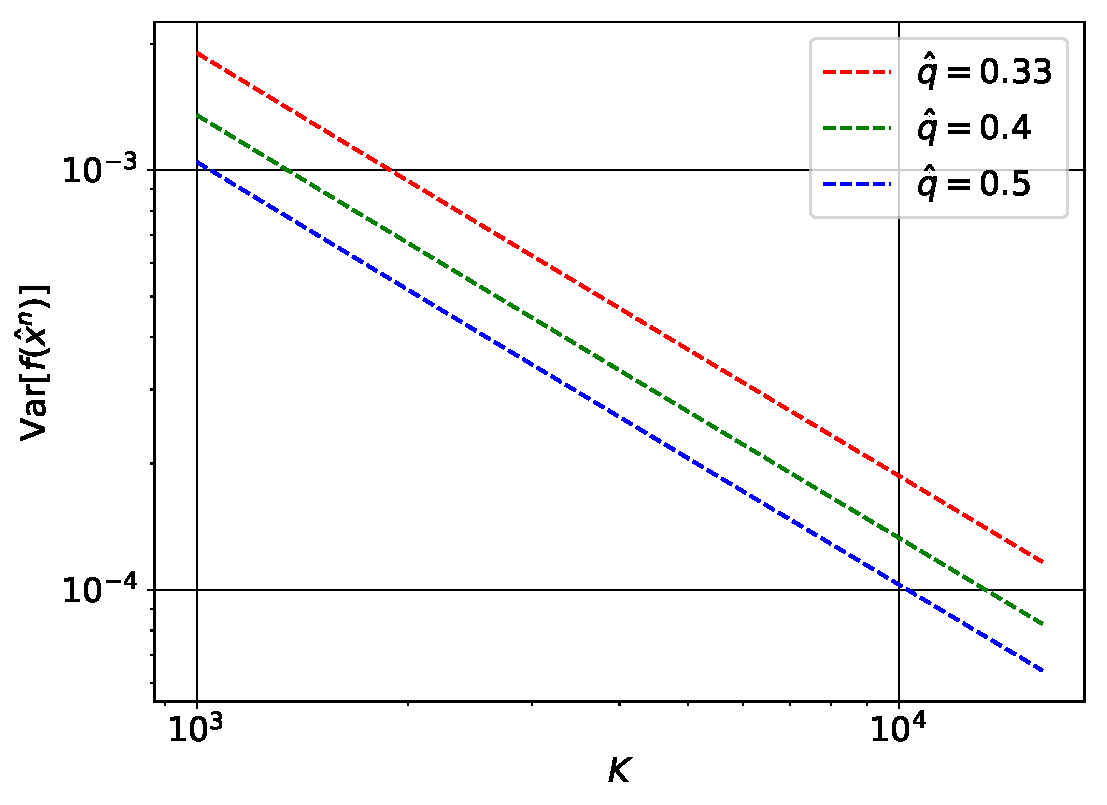
\includegraphics[width=0.8\linewidth]{../figure/fig3.pdf}
    % \begin{picture}(0,0)
    % \put(0,0){hogehoge}
    % \end{picture}
    \caption{The variance of the reference distribution computed based on Eq. (\ref{eq:sigma_C^2}) with $\hat{q}=0.33,\, 0.4$ and $0.5$ (Copyright(C)2020 IEICE, \cite{hikima2020} Figure 1)}
    \label{fig:1}
\end{figure}
%
\begin{table}[htbp]
  \centering
  \caption{$D_K(\hat{q})$ for different values of $\hat{q}$ and $K$}
  \begin{tabular}{ccccc} \hline
    $\hat{q}$ & $D_{10000}(\hat{q})$ & $D_{20000}(\hat{q})$ & $D_{30000}(\hat{q})$ & $D_{40000}(\hat{q})$  \\ \hline 
    $0.33$    & $1.867364$     & $1.865492$     & $1.864868$     & $1.864556$\\
    $0.4$     & $1.328692$     & $1.327430$     & $1.327009$     & $1.326799$\\
    $0.5$     & $1.028395$     & $1.027449$     & $1.027134$     & $1.026976$\\ \hline
  \end{tabular}
  \label{tab:1}
\end{table}
%
\begin{figure}[htbp]
  \centering
    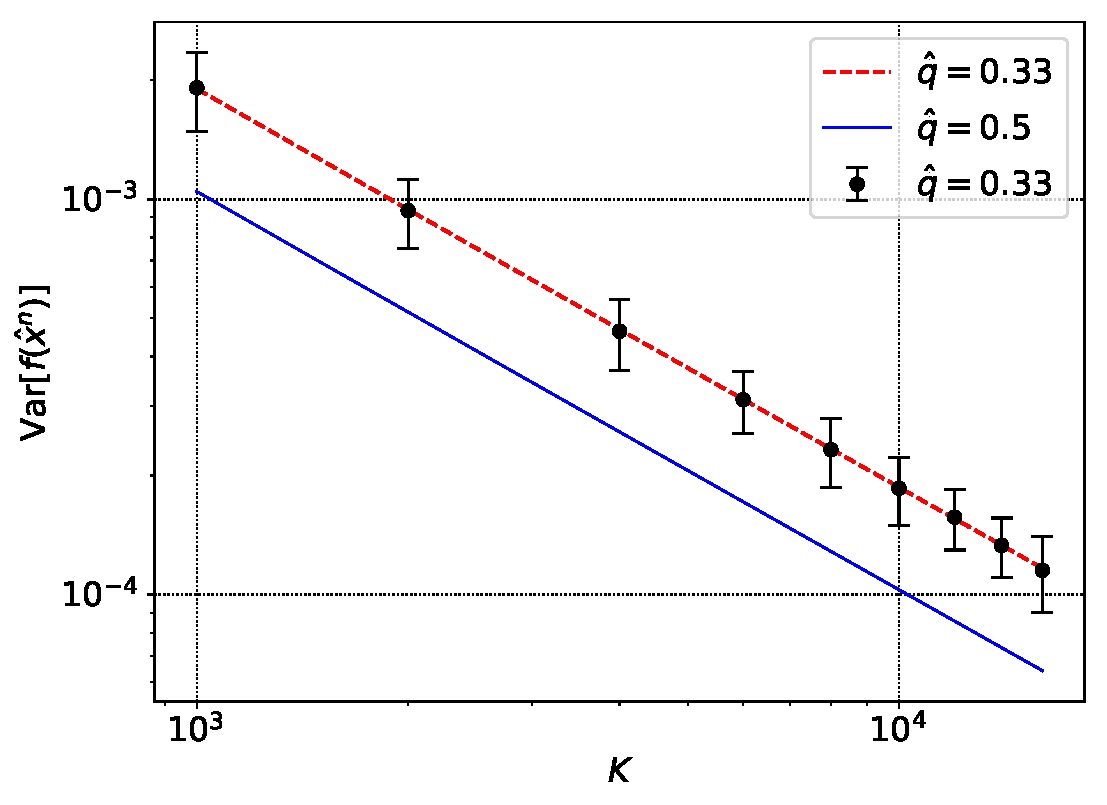
\includegraphics[width=0.7\linewidth]{../figure/fig4.pdf}
    \caption{The variance of the reference distribution computed in the experiment. The solid blue line and the broken red line are the variances computed based on Eq. (\ref{eq:sigma_C^2}) with $\hat{q}=0.5$ and $\hat{q}=0.33$, respectively. The block points show the arithmetic mean of the unbiased variance with $\hat{q}=0.33$ using Mersenne Twister. (Copyright(C)2020 IEICE, \cite{hikima2020} Figure 2)}
    \label{fig:2}
\end{figure}
%
%
%-----------------------------------------------------------------------------------------------%
%-----------------------------------------------------------------------------------------------%
%-----------------------------------------------------------------------------------------------%
\clearpage
\subsubsection{Experiment 2}\label{subsec:4-3}
We have seen that the variance of reference distribution of the highly sensitive test can be computed when $L=4$. We consider the case of $L=8$ and $\hat{q}=0.33$ which are recommended in \cite{yamamoto2016highly}. 
However, the computational cost for $L=8$ is too high to compute directly since the recommendation value for $K$ is $1000\times 2^8 = 256000$.
% Although the variance for $L=4$ can be computed directly using Eq. (\ref{eq:sigma_C^2}) since the recommendation value for $K$ is only $1000 \times 2^4 = 16000$, the computational cost for computing the variance for $L=8$ is too high, since the recommendation value for $K$ is $1000\times 2^8 = 256000$. 
To overcome the obstacle, we derive the fitted curve. 
%計算時間がかかるだけでなく計算の破綻を起こすことが確認された.そこで,得られているデータから近似曲線を求めることを考える.
% Note that the recommended value of $K$ is $K=1000\cdot 2^8$.
%
We approximate the variance of the reference distribution as
% The variance of reference distribution can be written as
\begin{align}\label{eq:approx_sigma}
  \sigma_{C,\hat{q}}(K)^2 = \frac{1}{K} \left( a + \frac{b}{K} \right),
\end{align}
where $a$ and $b$ are real valued constants. 
% Let $h(K) = a + \frac{b}{K}$. 
These constants can be obtained with any two points $(K_1, \sigma_{C,\hat{q}}(K_1)^2)$ and $(K_2, \sigma_{C,\hat{q}}(K_2)^2)$ by
\begin{align}\begin{split}\label{eq:keisuu_ab}
  % a &= \frac{1}{K_1-K_2} \left( K_1 h(K_1) - K_2 h(K_2)  \right), \\
  % b &= \frac{K_1K_2}{K_2-K_1} \left( h(K_1) - h(K_2)  \right).
  a &= \frac{1}{K_1-K_2} \left( K_1^2 \sigma_{C,\hat{q}}(K_1)^2 - K_2^2 \sigma_{C,\hat{q}}(K_2)^2  \right), \\
  b &= \frac{K_1K_2}{K_2-K_1} \left( K_1 \sigma_{C,\hat{q}}(K_1)^2 - K_2 \sigma_{C,\hat{q}}(K_2)^2 \right).
\end{split}\end{align}
%
Table \ref{tab:2} shows the pairs of $(a,b)$ obtained from $(K_1,K_2)=(40000,45000)$ and the standard deviation $\tilde{\sigma}_{C,\hat{q}}(K)$ for $K=1000\times2^L$ obtained from Eq. (\ref{eq:approx_sigma}).
%
% We adopt the result of $(K_1,K_2)=(40000,45000)$ and obtain the standard deviation for $K=1000\times 2^8$ as $\sigma_{C,0.33} (1000\times 2^8) = 0.0034886003$.
%
Figure \ref{eq:approx_sigma} show the fitted curve.
Using the fitted curve, we obtained the standard deviation for $K=1000\times 2^8$ as
\begin{align}\label{eq:proposed_value}
  \sigma_{C,0.33} (1000\times 2^8) = 0.003488600339.
\end{align}
%
%
\par
To confirm the accuracy of Eq. (\ref{eq:proposed_value}), we computed $\sigma_{C,0.33} (1000\times 2^8)$ using MT in 10 times. For each trial, we used $4\times 10^6$ pieces of binary sequences and set $Q=10\times 2^8$.
% We made an experiment described in Experiment 1 for choosing parameters as $L=8,\, Q=10\times 2^L,\,K=1000\times 2^L,\, \hat{q}=0.33,\, M=4\times 10^{6}$ and $N=10$. 
Table \ref{tab:2} and Figure \ref{fig:comparison_yamamoto} show the results of this experiment.
%
% We can see that the obtained value derived from Eqs. (\ref{eq:approx_sigma}) and (\ref{eq:keisuu_ab}) is closer to the empirical value than the value used in \cite{yamamoto2016highly}.
These results support that the value represented in Eq. (\ref{eq:proposed_value}) is more accurate than the value in previous study.
%
\begin{table}[htb]
  \centering
  \caption{The pairs of $(a,b)$ when $(K_1,K_2)=(40000,45000)$ and the standard deviation obtained from Eq. (\ref{eq:approx_sigma})}
  \begin{tabular}{ccc} \hline
    $(K_1,K_2)$      & $(a,b)$                            & $\tilde{\sigma}_{C,q}(K)$   \\ \hline 
    % $(20000,30000)$  & $(3.112120333856, 897.0609512838)$ & $0.003488611201$      \\
    % $(30000,40000)$  & $(3.112100900335, 897.6439269103)$ & $0.003488601597$      \\
    $(40000,45000)$  & $(3.112098237555, 897.7504381251)$ & $0.003488600339$      \\ \hline
    % $(45000,46000)$  & $(3.112097857417, 897.7675443506)$ & $0.003488600164$      \\ \hline
  \end{tabular}
  \label{tab:2}
\end{table}
%
\begin{figure}[htbp]
  \centering
    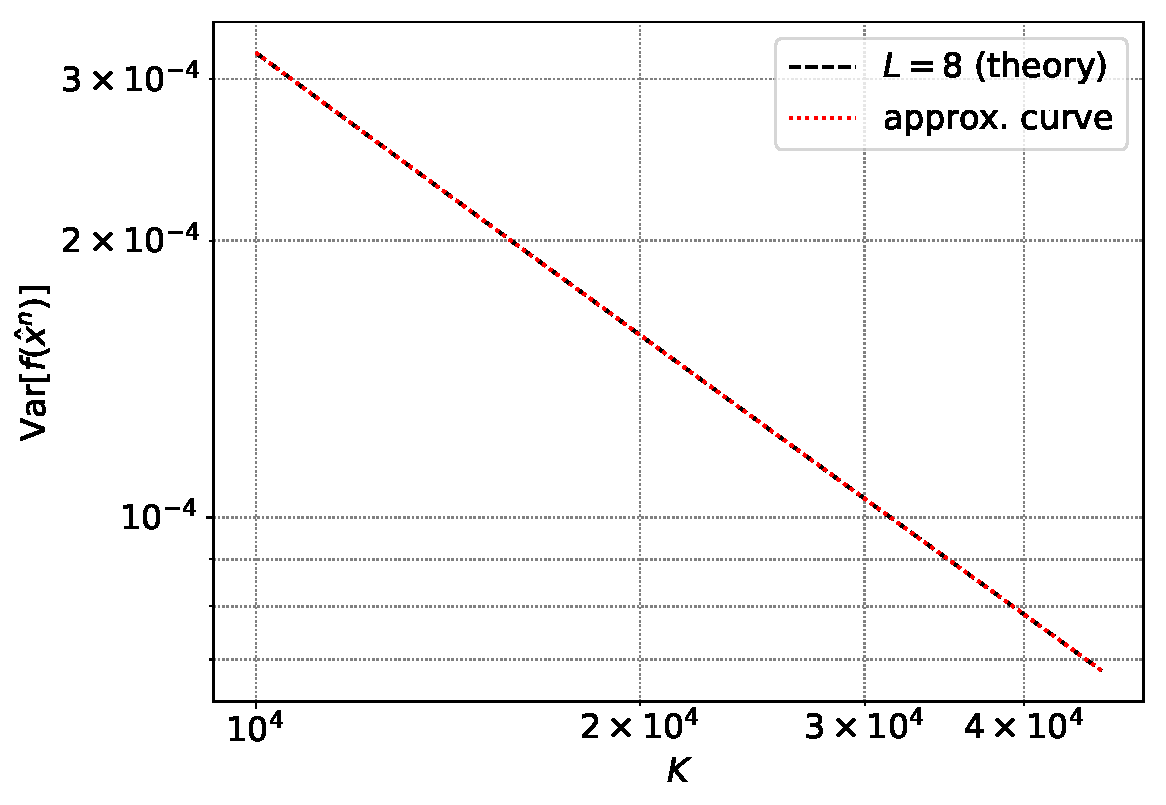
\includegraphics[width=0.7\linewidth]{../figure/approx_varf_L8_10000.pdf}
    \caption{The fitted curve}
    \label{fig:fitted}
\end{figure}
%
%
%-----------------------------------------------------------------------------------------------%
%
\begin{table}[tbp]
  \centering
  \caption{Value of $\sigma_{C,0.33}(1000\times 2^8)$ computed using the Mersenne Twister}
  \begin{tabular}{cc} \hline
    Trial No.   & $\sigma_{C,0.33}(1000\times 2^8)$           \\ \hline 
    1           & $0.00348911$       \\
    2           & $0.00348889$       \\
    3           & $0.00348837$       \\ 
    4           & $0.00349002$       \\ 
    5           & $0.00348612$       \\ 
    6           & $0.00348572$       \\ 
    7           & $0.00348889$       \\ 
    8           & $0.00348767$       \\ 
    9           & $0.00348672$       \\ 
    10          & $0.00349002$       \\ \hline 
    Total       & $0.00348816 \pm 2.44 \times 10^{-6}$ \\ \hline
  \end{tabular}
  \label{tab:3}
\end{table}
%
\begin{figure}[tbp]
  \centering
  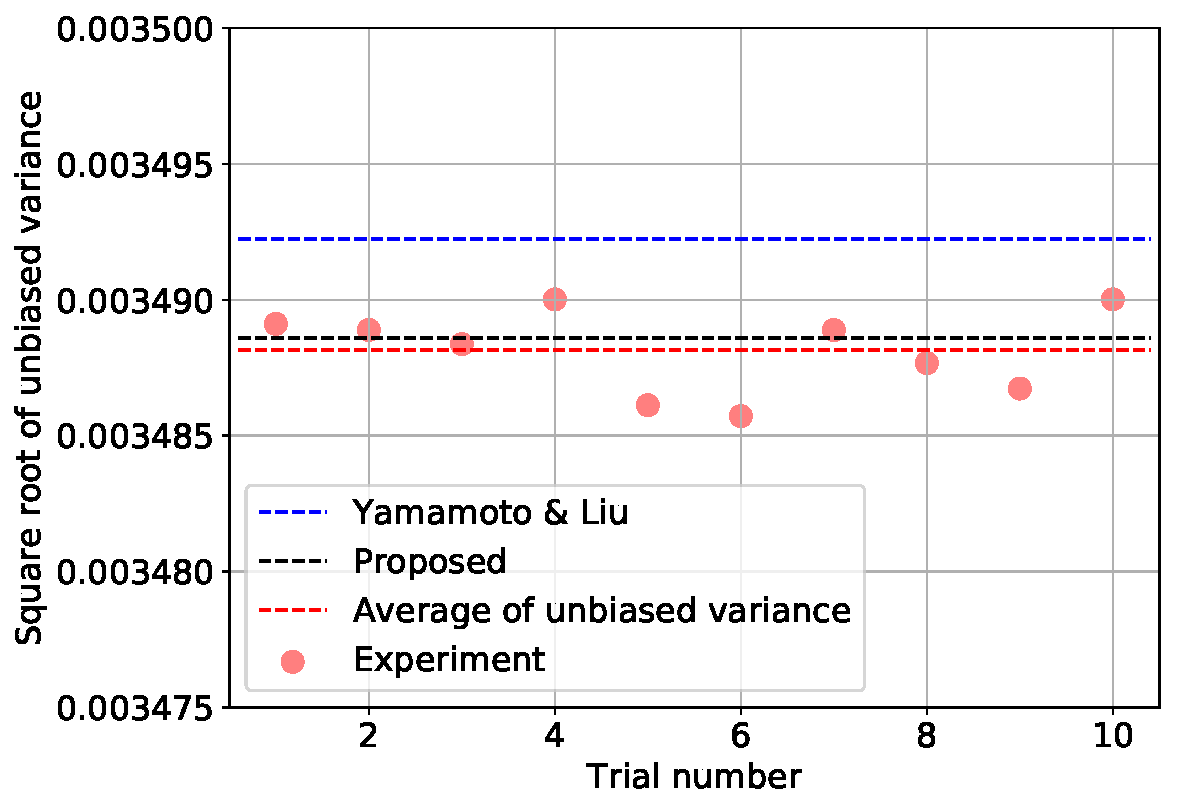
\includegraphics[width=0.7\linewidth]{../figure/unbiased_variance.pdf}
  % \caption{Plots of values of square root of unbiased variance computed using the Mersenne Twister. The blue broken line is the value given in \cite{yamamoto2016highly}, the black broken line is the value given in the subsection \ref{subsec:4-2}, and the red broken line is the average of square root of unbiased variance.}
  \caption{The variance $\sigma_{C,0.33}(1000\times 2^8)$. Each point shows an unbiased variance derived empirically and the red broken line shows the arithmetic mean. The blue broken line shows the value given in \cite{yamamoto2016highly}. The black broken line represented in Eq. (\ref{eq:proposed_value}).}
  % \caption{The variance of reference distribution for $L=4$ and $\hat{q}=0.33$.}
  \label{fig:comparison_yamamoto}
\end{figure}
%-----------------------------------------------------------------------------------------------%
\clearpage
\subsubsection{Experiment 3}
%このセクションでは,得られた参照分布の分散を用いて検定を行なった場合と,先行研究で与えられている数値を使った場合の違いについて考察する.
We investigated the difference between the value derived in Experiment 2 and the value given in \cite{yamamoto2016highly}. In the follows, we refer to the value represented in Eq. (\ref{eq:proposed_value}) as proposed value and the value given in \cite{yamamoto2016highly} as Yamamoto's value. We used MT \cite{matsumoto1998mersenne} and AES-128 CTR \cite{rijmen2001advanced} as pseudo random number generators. 
\par
Each test was performed for $10^5$ sequences of length $n=2068480$-bit. We divided them into $100$ sets of $1000$ sequences. We assigned pass or rejected for each set based on two-level tests, ``proportion test'' and ``uniformity test'', described in subsection \ref{subsec:1-2}.
% These sequences are associated with pass or rejection assigned for each set based on two-level tests, ``proportion test'' and ``uniformity test'', described in subsection \ref{subsec:1-2}. 
%
Recall that the significance level for uniformity test is $0.0001$. 
Since the significance level for uniformity test is so small that we cannot observe the difference, we executed uniformity test with the significance levels $0.01$ and $0.05$.
% We executed the tests with several significance levels since significance level is so small that we cannot observe the difference. 
% We also additionally perform the Proportion test with two-sigma significance as well as three-sigma significance.
By the same reason, we additionally performed proportion test with $\xi=2$ as well as $\xi=3$.
% two-sigma significance as well as three-sigma significance.
\par
The results of Experiment 2 imply that more sequences should be used to observe the differences between the highly sensitive test with the proposed value and the test with the Yamamoto's value. We cannot expect to get any meaningful results because there are some approximation errors. For instance, we assume that the p-value takes any real value in $[0,1]$, but practically it can take only discrete values. When we use an enormous number of sequences, we cannot avoid the effect of such errors.
%
Thus, the purpose of the experiments is only to confirm that the proposed value does not cause any problem in practical situation.
\par
Tables \ref{tab:proportion_1} and \ref{tab:proportion_2} show the results of proportion test with $\xi=3$ and with $\xi=2$, respectively. Tables \ref{tab:uniformity_1}, \ref{tab:uniformity_2} and \ref{tab:uniformity_3} show the results of uniformity test with the significance levels $0.0001$, $0.01$ and $0.05$, respectively. Note that ``MT/AES'' means that a tested sequence is generated by Mersenne Twister and AES-128 CTR is used for flipping each bit. ``AES/MT'' and ``AES/AES'' are defined in the same manner.
% \par
% If the highly sensitive test with our proposed value accepts or rejects much more sets, it may indicate that our proposed value is problematic. However, there is no such cases according to Tables \ref{tab:proportion_1}, \ref{tab:proportion_2}, \ref{tab:uniformity_1}, \ref{tab:uniformity_2} and \ref{tab:uniformity_3}, which supports our proposed value is robust.
The results in Tables \ref{tab:proportion_1}, \ref{tab:proportion_2}, \ref{tab:uniformity_1}, \ref{tab:uniformity_2} and \ref{tab:uniformity_3} support that the proposed value is robust.
%-----------------------------------------------------------------------------------------------%
\begin{table}[htb]
  \centering
  \caption{Number of sets rejected by proportion test with $\xi=3$}
  \begin{tabular}{ccc} \hline
              & Yamamoto \cite{yamamoto2016highly}  & Proposed \\ \hline 
    MT/AES    & 0         & 0        \\
    AES/MT    & 0         & 0        \\
    AES/AES   & 0         & 0        \\ \hline 
  \end{tabular}
  \label{tab:proportion_1}
\end{table}
%-----------------------------------------------------------------------------------------------%
\begin{table}[htb]
  \centering
  \caption{Number of sets rejected by proportion test with $\xi=2$}
  \begin{tabular}{ccc} \hline
              & Yamamoto \cite{yamamoto2016highly} & Proposed \\ \hline 
    MT/AES    & 2         & 3        \\
    AES/MT    & 4         & 4        \\
    AES/AES   & 6         & 6        \\ \hline 
  \end{tabular}
  \label{tab:proportion_2}
\end{table}
%-----------------------------------------------------------------------------------------------%
\begin{table}[t]
  \centering
  \caption{Number of sets rejected by uniformity test with the significance level $0.0001$}
  \begin{tabular}{ccc} \hline
              & Yamamoto \cite{yamamoto2016highly} & Proposed \\ \hline 
    MT/AES    & 0         & 0        \\
    AES/MT    & 0         & 0        \\
    AES/AES   & 0         & 0        \\ \hline 
  \end{tabular}
  \label{tab:uniformity_1}
\end{table}
%-----------------------------------------------------------------------------------------------%
\begin{table}[t]
  \centering
  \caption{Number of sets rejected by uniformity test with the significance level $0.01$}
  \begin{tabular}{ccc} \hline
              & Yamamoto \cite{yamamoto2016highly} & Proposed \\ \hline 
    MT/AES    & 0         & 0        \\
    AES/MT    & 0         & 1        \\
    AES/AES   & 0         & 0        \\ \hline 
  \end{tabular}
  \label{tab:uniformity_2}
\end{table}
%-----------------------------------------------------------------------------------------------%
\begin{table}[t]
  \centering
  \caption{Number of sets rejected by uniformity test with the significance level $0.05$}
  \begin{tabular}{ccc} \hline
              & Yamamoto \cite{yamamoto2016highly} & Proposed \\ \hline 
    MT/AES    & 2         & 2        \\
    AES/MT    & 3         & 6        \\
    AES/AES   & 4         & 5        \\ \hline 
  \end{tabular}
  \label{tab:uniformity_3}
\end{table}
%-----------------------------------------------------------------------------------------------%
%-----------------------------------------------------------------------------------------------%
%-----------------------------------------------------------------------------------------------%
%-----------------------------------------------------------------------------------------------%
%-----------------------------------------------------------------------------------------------%
%-----------------------------------------------------------------------------------------------%
%-----------------------------------------------------------------------------------------------%
%-----------------------------------------------------------------------------------------------%
%-----------------------------------------------------------------------------------------------%
%-----------------------------------------------------------------------------------------------%
%-----------------------------------------------------------------------------------------------%
%-----------------------------------------------------------------------------------------------%
\clearpage
\section{Conclusion}\label{sec:conclusion}
%highly sensitive testの帰無仮説の下での参照分布を理論的に導出した.
In this thesis, we have theoretically derived the variance for the reference distribution of highly sensitive universal statistical test. 
%
In deriving process, the marginal distribution of $A_n$ and the joint distribution of $(A_n,A_{n+k})$ have been derived theoretically with the fact that the sequence of $\{A_k\}_{k=1}^{K}$ can be considered as stationary ergodic under the assumption of $Q\to\infty$. 
%
We have shown that the value of the variance can be numerically computed for the block size $L=4$.
%
Because of computational cost, we used an fitted curve to get the numerical value of the variance for $L=8$.
%
% We also have derived the approximated curve in order to obtain the variance when $L=8$. 
Since the value obtained by the fitted curve may have some error, we have compared with the unbiased variance computed from binary sequences generated by a pseudo random number generator. By this experiment, we have confirmed that the value obtained from the fitted curve is more consistent with the experimental result than the existing value which has been obtained by a numerical experiment.
%
We can state that the value of the variance in this thesis is superior subject to the existing one. 
%
Thus, we recommend that the value obtained in this thesis should be used when the highly sensitive universal statistical test is performed so that randomness of binary sequences can be tested more precisely.
%
%-- Acknowledgments -------------------------------------------------------------
\clearpage
\acknowledgment
The author would like to express his sincere gratitude to Professor Ken Umeno for his guidance and helpful advice.
%
I would also like to express my appreciation for Assistant Professor Atsushi Iwasaki for his support and encouragement in keeping my progress.
%
\par
Furthermore, I would like to extend my thanks to the member of Physical Statistical Laboratory for their support during my study. 
%
I would especially grateful to Dr. Hirofumi Tsuda and Mr. Shinji Kakinaka for their extended discussions and valuable suggestions which have greatly contributed to the improvement of this thesis.
%
\par
Finally, I wish to thank my family for their support and encouragement throughout my study.
%
%-- References ------------------------------------------------------------------
\clearpage
\addcontentsline{toc}{section}{\refname} % Add to the table of contents.
                                         % Delete if you use chapter option.
\bibliographystyle{ieeetr}
\bibliography{cite}
%
%-- Appendix ---------------------------------------------------------------------
%%% If you don't need appendices, delete the below.
\clearpage
\appendix
\section{Proof of $C=-\frac{\ln 2}{\gamma}$}\label{appendix:A}
In this appendix, we provide the proof of the following theorem.
\begin{theorem}
For any $x\in(0,1)$, we have the following relation
\begin{align}
	\lim_{x\to 0+} \left[ v(x) + \log_2 x \right] = -\frac{\gamma}{\ln 2} = -0.832746\cdots,
\end{align}
where
\begin{align}
	v(x) = x\sum_{i=1}^{\infty} (1-x)^{i-1}\log_2 i,
\end{align}
and $\gamma$ is Euler's constant defined by
\begin{align}\label{eq:gamma_def}
	\gamma := \lim_{n\to\infty}\left(\sum_{i=1}^{n} \frac{1}{i}-\ln n\right).
\end{align}
\end{theorem}
%
\begin{proof}
Let $s=1-x$. We have
\begin{align}\begin{split}
	v(1-s) + \log_2 (1-s) 
	&= (1-s)\sum_{i=1}^{\infty} s^{i-1}\log_2 i + \log_2 (1-s) \\
	&= \frac{1}{\ln2} \left\{ (1-s) \sum_{i=1}^{\infty}s^{i-1}\ln i + \ln(1-s) \right\} \\
	&= \frac{1}{\ln2} \left\{ (1-s)\times \frac{1}{1-s} \sum_{i=1}^{\infty}s^{i} \times \ln \frac{i+1}{i} - \sum_{i=1}^{\infty} \frac{s^i}{i} \right\} \\
	&= \frac{1}{\ln2} \sum_{i=1}^{\infty}s^{i} \left\{ \ln \left(1+\frac{1}{i}\right) - \frac{1}{i} \right\}.
\end{split}\end{align}
From the above equations, we have
\begin{align}\begin{split}
	\lim_{s\to 1-} \left[ v(1-s) + \log_2 (1-s) \right] 
	&=\frac{1}{\ln2} \lim_{s\to 1-} \left[ \sum_{i=1}^{\infty} s^{i} \left\{ \ln \left(1+\frac{1}{i}\right) - \frac{1}{i} \right\} \right]\\
	&=\frac{1}{\ln2} \sum_{i=1}^{\infty} \lim_{s\to 1-} \left[ s^{i} \left\{ \ln \left(1+\frac{1}{i}\right) - \frac{1}{i} \right\} \right] \\
	&=\frac{1}{\ln2} \sum_{i=1}^{\infty}\left\{ \ln \left(1+\frac{1}{i}\right) - \frac{1}{i} \right\}.
\end{split}\end{align}
For the derivation of the second equation, we have used the fact that the infinite series converges absolutely which allows us to exchange the limits. 
%
Since $\ln n$ can be written as 
\begin{align}
	\ln n = \ln \left( \frac{2}{1}\cdot\frac{3}{2}\cdot\frac{4}{3}\cdot\cdots\frac{n}{n-1}\right) = \sum_{k=1}^{n-1}\ln\left(1+\frac{1}{k}\right),
\end{align}
Euler's constant $\gamma$ defined by Eq. (\ref{eq:gamma_def}) can also be represented as
\begin{align}\begin{split}
	\gamma &= \lim_{n\to\infty} \left[ \sum_{k=1}^{n-1}\left\{ \frac{1}{k} - \ln \left(1+\frac{1}{k}\right)\right\} + \frac{1}{n} \right] \\
	&=\sum_{n=1}^{\infty}\left\{ \frac{1}{n} - \ln \left(1+\frac{1}{n}\right) \right\}.
\end{split}\end{align}
Therefore, we arrive at the following result
\begin{align}
	\lim_{s\to 1-} \left[ v(1-s) + \log_2 (1-s) \right]  =- \frac{\gamma}{\ln 2}.
\end{align}
The theorem is obtained if we substitute $s$ into $1-x$.
\end{proof}
\clearpage
\newpage
\section{Exploration of the covariance given in Eq. (\ref{eq:covariance_g_g})}\label{appendix:B}
In this appendix, we explore the covariance given in Eq. (\ref{eq:covariance_g_g}) to calculate the value more efficiently by computational experiments. Notice that the covariance is written as 
\begin{align}\label{eq:cov_saikei}
	\mathrm{Cov}[g(A_n),\, g(A_{n+k})] 
	= \sum_{i=1}^{\infty} \sum_{j=1}^{\infty} g(i) g(j) \mathrm{Pr} \left[ A_n=i,\,A_{n+k}=j \right] - \{L\times H(\hat{q})\}^2,
\end{align}
where $g$ is given in Eq. (\ref{eq:function_g}), $\mathrm{Pr} \left[ A_n=i,\,A_{n+k}=j \right]$ is given in Eq. (\ref{eq:joint_distribution}), and $H$ is a binary entropy function.
%
Since the term $\{L\times H(\hat{q})\}^2$ is irrelevant to an infinite series, we write the first term of the right hand side (r.h.s.) of Eq. (\ref{eq:cov_saikei}) as
%
\begin{align}\label{eq:Sk}
	\overline{S}_{k} := \sum_{i=1}^{\infty} \sum_{j=1}^{\infty} g(i) g(j) \mathrm{Pr} \left[ A_n=i,\,A_{n+k}=j \right].
\end{align}
%
Firstly, we show the following Lemma concerning an infinite series to calculate the value expressed Eq. (\ref{eq:Sk}). 
%
\begin{lemma}\label{lemma:1}
% abcdefghijklmnopqrstuvwxyz
For any $z \in (0,1)$, the following relation holds
\begin{align}\label{eq:infinite_series}
	\sum_{i=1}^{\infty} g(i) \times (1-z)^i = -\frac{1}{\ln 2} \times \frac{1-z}{z} \times \ln z,
\end{align}
where
\begin{align}
	g(m) = (\log_2 \mathrm{e}) \sum_{k=1}^{m-1} \frac{1}{k}.
\end{align}
\end{lemma}
%-----------------------------------------------------------------------------------------------%
\begin{proof}
Let $t=1-z$, and $\overline{S}$ be the left hand side of Eq. (\ref{eq:infinite_series}), that is,
\begin{align}\begin{split}\label{eq:S}
  \overline{S} &= \sum_{i=1}^{\infty} g(i) \times t^i \\
    % \Leftrightarrow S &= g(1)\times A +  \sum_{i=2}^{\infty} g(i) \times A^{i} \label{eq:S}.
    &= g(1)\times t +  \sum_{i=2}^{\infty} g(i) \times t^{i}.
\end{split}\end{align}
Multiplying the both sides of Eq. (\ref{eq:S}) by $t(\neq 0)$, we obtain the following relation
\begin{align}\begin{split}\label{eq:AS}
  t\times \overline{S} &= \sum_{i=1}^{\infty} g(i) \times t^{i+1} \\
  &= \sum_{i=2}^{\infty} g(i-1) \times t^{i}.
\end{split}\end{align}
Subtracting Eq. (\ref{eq:AS}) from Eq. (\ref{eq:S}), we obtain the following relation
\begin{align}\begin{split}\label{eq:(1-A)S}
  (1-t)\overline{S} &= g(1)\times t^{1} + \sum_{i=2}^{\infty} \left\{ g(i)-g(i-1) \right\} \times t^{i} \\
  &=0 + \sum_{i=2}^{\infty} (\log_2 \mathrm{e}) \times \frac{1}{i-1} \times t^{i} \\
  &=(\log_2 \mathrm{e})\times t \times \sum_{i=1}^{\infty} \frac{t^{i}}{i} \\
  &=(\log_2 \mathrm{e})\times t \times \left\{ - \ln (1-t) \right\}.
\end{split}\end{align}
To obtain the last equality in the above equations, we have used the Taylor series for $|t| < 1$.
Dividing both sides of Eq. (\ref{eq:(1-A)S}) by $1-t (\neq 0)$, we arrive at the following result
\begin{align}
  \overline{S} &= -\frac{1}{\ln 2} \times \frac{t}{1-t} \times \ln (1-t).
\end{align}
The lemma is obtained if we substitute $t$ into $1-z$.
\end{proof}
%-----------------------------------------------------------------------------------------------%
%-----------------------------------------------------------------------------------------------%
%-----------------------------------------------------------------------------------------------%
\par
In the next place, we calculate the value given in Eq. (\ref{eq:Sk}) more in details.
\subsection{Case of $1 \leq j \leq k-1$}
For $1 \leq j \leq k-1$, Eq. (\ref{eq:Sk}) is written as
\begin{align}\begin{split}
  \overline{S}_{k} 
  &:= \sum_{i=1}^{\infty} \sum_{j=1}^{k-1} g(i) g(j) \mathrm{Pr} \left[ A_n=i,\,A_{n+k}=j \right] \\
  &= \sum_{i=1}^{\infty} \sum_{j=1}^{k-1} g(i) g(j) \left( \sum_{r=0}^{L} \binom{L}{r}w_r^2 (1-w_r)^{i-1} \right) \times \left( \sum_{r=0}^{L} \binom{L}{r}w_r^2 (1-w_r)^{j-1} \right) \\ 
  &= \sum_{r=0}^{L} \left\{\binom{L}{r} \frac{w_r^2}{1-w_r} \sum_{i=1}^{\infty} g(i)(1-w_r)^{i} \right\}
  \times \sum_{r=0}^{L} \left\{ \binom{L}{r} \frac{w_r^2}{1-w_r} \sum_{j=1}^{k-1} g(j)(1-w_r)^{j} \right\}.
\end{split}\end{align}
From Lemma \ref{lemma:1}, the infinite series of $i$ in the above equations is written as
\begin{align}
	\sum_{i=1}^{\infty} g(i) (1 - w_r)^{i} = - \frac{1}{\ln 2} \times \frac{1-w_r}{w_r}\times\ln w_r.
\end{align}
%
Therefore, we obtain the following relation
\begin{align}\begin{split}
  \overline{S}_{k}
  =& \sum_{r=0}^{L} \left\{ \dbinom{L}{r} \frac{w_r^2}{1-w_r}  \times \left(- \frac{1}{\ln 2} \times \frac{1-w_r}{w_r}\times\ln w_r \right) \right\} \\
  &\times \sum_{r=0}^{L} \left\{ \dbinom{L}{r} \frac{w_r^2}{1-w_r} \times \sum_{j=1}^{k-1} (1-w_r)^{j} \right\} \\
  =&-\frac{1}{\ln 2}\sum_{r=0}^{L} \left\{ \dbinom{L}{r} w_r \ln w_r \right\} \times \sum_{r=0}^{L} \left\{ \dbinom{L}{r} \frac{w_r^2}{1-w_r} \sum_{j=1}^{k-1} (1-w_r)^{j} \right\}.
\end{split}\end{align}
%
\subsection{Case of $j=k$}
In the case of $j=k$, Eq. (\ref{eq:Sk}) is written as
\begin{align}\begin{split}\label{eq:app_case2}
  \overline{S}_{k} 
  &= \sum_{i=1}^{\infty} g(i) \sum_{r=0}^{L} \binom{L}{r} w_r^3 (1-w_r)^{k+i-2} \sum_{j \in \{k\}} g(j)\\
  &= \sum_{r=0}^{L} \binom{L}{r} w_r^3 (1-w_r)^{k-2} \sum_{i=1}^{\infty} g(i) (1-w_r)^{i} \times g(k) \\
  &= g(k) \times \sum_{r=0}^{L} \binom{L}{r} w_r^3 (1-w_r)^{k-2} \left( -\frac{1}{\ln 2} \times \frac{1-w_{r}}{w_{r}} \times \ln w_{r} \right) \\
  &= -\frac{g(k)}{\ln 2} \times \sum_{r=0}^{L} \binom{L}{r} w_r^2 (1-w_r)^{k-1} \ln w_{r}.
\end{split}\end{align}
The third equation in Eq. (\ref{eq:app_case2}) has been obtained from Lemma \ref{lemma:1}.
%-----------------------------------------------------------------------------------------------%
%-----------------------------------------------------------------------------------------------%
%-----------------------------------------------------------------------------------------------%
\subsection{Case of $k+1 \leq j \leq k+i-1$}
Recall that the joint distribution for $k+1 \leq j \leq k+i-1$ is written as
\begin{align}\begin{split}
	\mathrm{Pr}[A_n=i,\, A_{n+k}=j] 
	=& \sum_{r_1=0}^{L} \sum_{r_2 \neq r_1} \binom{L}{r_1}\binom{L}{r_2}\mathrm{Pr}[e_3(b_1,b_2)] \\
	&+ \sum_{r_1=0}^{L} \sum_{r_2 \in \{r_1\}} \binom{L}{r_1}\left\{\binom{L}{r_1}-1\right\}\mathrm{Pr}[e_3(b_1,b_2)],
\end{split}\end{align}
where $\mathrm{Pr}[e_3(b_1,b_2)]$ is expressed as
\begin{align}\begin{split}
	\mathrm{Pr}[e_3(b_1,b_2)]
  =& w_{r_1}^2  \times w_{r_2}^2 
  \times (1-w_{r_1})^{i-j+k-1} 
  \times (1-w_{r_1}-w_{r_2})^{j-k-1}
  \times (1-w_{r_2})^{k-1} \\
  =&\phi_k(r_1,r_2)\times (1-w_{r_1})^{i} \times \left(1-\frac{w_{r_2}}{1-w_{r_1}} \right)^{j},
\end{split}\end{align}
%
where
\begin{align}\label{eq:phi_k}
	\phi_k(r_1,r_2) = w_{r_1}^2 w_{r_2}^2 
  	(1-w_{r_1})^{k-1} 
  	(1-w_{r_1}-w_{r_2})^{-k-1}
  	(1-w_{r_2})^{k-1}.
\end{align}
%
Then, Eq. (\ref{eq:Sk}) is expressed as
\begin{align}\begin{split}\label{eq:Sk_case3}
	\overline{S}_k 
	=& \sum_{i=1}^{\infty}\sum_{j=k+1}^{k+i-1} g(i)g(j) \sum_{r_1=0}^{L} \sum_{r_2 \neq r_1} \binom{L}{r_1}\binom{L}{r_2}\mathrm{Pr}[e_3(b_1,b_2)]\\ 
	&+ \sum_{i=1}^{\infty}\sum_{j=k+1}^{k+i-1} g(i)g(j) \sum_{r_1=0}^{L} \sum_{r_2 \in \{r_1\}} \binom{L}{r_1} \left\{\binom{L}{r_1}-1 \right\}\mathrm{Pr}[e_3(b_1,b_2)].
\end{split}\end{align}
%
Now, we consider the first term in r.h.s. of Eq. (\ref{eq:Sk_case3}). Let $\overline{A}_1$ be this term of Eq. (\ref{eq:Sk_case3}). We have
\begin{align}\begin{split}\label{eq:A_1}
	\overline{A}_1
	&=\sum_{i=1}^{\infty}\sum_{j=k+1}^{k+i-1} g(i)g(j) \sum_{r_1=0}^{L} \sum_{r_2 \neq r_1} \binom{L}{r_1}\binom{L}{r_2}\mathrm{Pr}[e_3(b_1,b_2)] \\
	&=\sum_{r_1=0}^{L} \sum_{r_2 \neq r_1} \binom{L}{r_1}\binom{L}{r_2}\phi_k(r_1,r_2)
	\sum_{i=1}^{\infty} \sum_{j=1}^{k+i-1} g(i)g(j)(1-w_{r_1})^{i} \times \left(1-\frac{w_{r_2}}{1-w_{r_1}} \right)^{j} \\
	&=\sum_{r_1=0}^{L} \sum_{r_2 \neq r_1} \binom{L}{r_1}\binom{L}{r_2}\phi_k(r_1,r_2)
	\sum_{j=k+1}^{\infty} \sum_{i=k+1}^{k+i-1} g(i)g(j)(1-w_{r_1})^{i} \times \left(1-\frac{w_{r_2}}{1-w_{r_1}} \right)^{j} \\
	&=\sum_{r_1=0}^{L} \sum_{r_2 \neq r_1} \binom{L}{r_1}\binom{L}{r_2}\phi_k(r_1,r_2)
	\sum_{j=k+1}^{\infty} \left\{ g(j) \left(1-\frac{w_{r_2}}{1-w_{r_1}} \right)^{j} \times \sum_{i=j-k+1}^{\infty} g(i)(1-w_{r_1})^{i} \right\}.
\end{split}\end{align}
In the course of the derivation of the above relations, the second equation has been obtained from Eq. (\ref{eq:phi_k}). The third equation has been obtained by exchanging the summation over $i$ and $j$.
%
Then, the infinite series with respect to $i$ in the last equation of Eq. (\ref{eq:A_1}) can be calculated as
\begin{align}\begin{split}
	\sum_{i=j-k+1}^{\infty} g(i)(1-w_{r_1})^{i} 
	&= \sum_{i=1}^{\infty} g(i)(1-w_{r_1})^{i} - \sum_{i=1}^{j-k} g(i)(1-w_{r_1})^{i} \\
	&= -\frac{1}{\ln 2} \times \frac{1-w_{r_1}}{w_{r_1}} \times \ln w_{r_1} - \sum_{i=1}^{j-k} g(i)(1-w_{r_1})^{i}.
\end{split}\end{align}
In the above relations, we have used the result of Lemma \ref{lemma:1}.
Hence, the first term in r.h.s. of Eq. (\ref{eq:Sk_case3}) can be expressed as
\begin{align}
	\overline{A}_1 
	=& \sum_{r_1=0}^{L} \sum_{r_2 \neq r_1} \binom{L}{r_1}\binom{L}{r_2}\phi_k(r_1,r_2)\\
	&\times\sum_{j=k+1}^{\infty} \left[ g(j) \left(1-\frac{w_{r_2}}{1-w_{r_1}} \right)^{j} \times \left\{ -\frac{1}{\ln 2} \times \frac{1-w_{r_1}}{w_{r_1}} \times \ln w_{r_1} - \sum_{i=1}^{j-k} g(i)(1-w_{r_1})^{i} \right\} \right].
\end{align}
We can derive the second term in r.h.s. of Eq. (\ref{eq:Sk_case3}) in the same way as the first term. Let $\overline{A}_2$ be the second term of Eq. (\ref{eq:Sk_case3}). Then, we have
\begin{align}\begin{split}
	\overline{A}_2 =& \sum_{r_1=0}^{L} \sum_{r_2 \in \{r_1\}} \binom{L}{r_1}\left\{\binom{L}{r_1}-1\right\} \phi(r_1,r_2) \\
	&\times\sum_{j=k+1}^{\infty} \left[ g(j) \left(1-\frac{w_{r_2}}{1-w_{r_1}} \right)^{j} \times \left\{ -\frac{1}{\ln 2} \times \frac{1-w_{r_1}}{w_{r_1}} \times \ln w_{r_1} - \sum_{i=1}^{j-k} g(i)(1-w_{r_1})^{i} \right\} \right].
\end{split}\end{align}
%
Therefore, Eq. (\ref{eq:Sk_case3}) can be written as
\begin{align}\begin{split}
	\overline{S}_k =& \overline{A}_1 + \overline{A}_2 \\
	=& \sum_{r_1=0}^{L} \sum_{r_2 \neq r_1} \binom{L}{r_1}\binom{L}{r_2}\phi_k(r_1,r_2)\\
	&\times\sum_{j=k+1}^{\infty} \left[ g(j) \left(1-\frac{w_{r_2}}{1-w_{r_1}} \right)^{j} \times \left\{ -\frac{1}{\ln 2} \times \frac{1-w_{r_1}}{w_{r_1}} \times \ln w_{r_1} - \sum_{i=1}^{j-k} g(i)(1-w_{r_1})^{i} \right\} \right] \\
	&+\sum_{r_1=0}^{L} \sum_{r_2 \in \{r_1\}} \binom{L}{r_1}\left\{\binom{L}{r_1}-1\right\} \phi(r_1,r_2) \\
	&\times\sum_{j=k+1}^{\infty} \left[ g(j) \left(1-\frac{w_{r_2}}{1-w_{r_1}} \right)^{j} \times \left\{ -\frac{1}{\ln 2} 
	\times \frac{1-w_{r_1}}{w_{r_1}} \times \ln w_{r_1} - \sum_{i=1}^{j-k} g(i)(1-w_{r_1})^{i} \right\} \right],
\end{split}\end{align}
where $\phi_k(r_1,r_2)$ is given in Eq. (\ref{eq:phi_k}).
%-----------------------------------------------------------------------------------------------%
%-----------------------------------------------------------------------------------------------%
%-----------------------------------------------------------------------------------------------%
\subsection{Case of $j=k+i$}
Equation (\ref{eq:Sk}) in the case of $j=k+i$ is equal to $0$ from Eq. (\ref{eq:joint_distribution}).
%-----------------------------------------------------------------------------------------------%
%-----------------------------------------------------------------------------------------------%
%-----------------------------------------------------------------------------------------------%
\subsection{Case of $j \geq k+i+1$}
%--------------------------------------------------------------------------------%
Recall that the joint distribution for $j \geq k+i+1$ is written as
\begin{align}\begin{split}
  \mathrm{Pr}[A_n=i,\, A_{n+k}=j] 
  =& \sum_{r_1=0}^{L} \sum_{r_2 \neq r_1} \binom{L}{r_1}\binom{L}{r_2}\mathrm{Pr}[e_5(b_1,b_2)] \\
  &+ \sum_{r_1=0}^{L} \sum_{r_2 \in \{r_1\}} \binom{L}{r_1}\left\{\binom{L}{r_1}-1\right\}\mathrm{Pr}[e_5(b_1,b_2)],
\end{split}\end{align}
where $\mathrm{Pr}[e_5(b_1,b_2)]$ is expressed as
\begin{align}\begin{split}
  \mathrm{Pr}[e_5(b_1,b_2)]
  =& w_{r_1}^2  \times w_{r_2}^2 
  \times (1-w_{r_1})^{-i+j-k-1} 
  \times (1-w_{r_1}-w_{r_2})^{i-1}
  \times (1-w_{r_1})^{k-1} \\
  =&\psi_k(r_1,r_2)\times \left(1-\frac{w_{r_2}}{1-w_{r_1}} \right)^{i} \times (1-w_{r_1})^j,
\end{split}\end{align}
%
where
\begin{align}\begin{split}\label{eq:psi_k}
  \psi_k(r_1,r_2) 
  &= w_{r_1}^2 w_{r_2}^2 
    (1-w_{r_1})^{-k-1} 
    (1-w_{r_1}-w_{r_2})^{-1}
    (1-w_{r_1})^{k-1} \\
  &= w_{r_1}^2 w_{r_2}^2 (1-w_{r_1})^{-2} (1-w_{r_1}-w_{r_2})^{-1}.
\end{split}\end{align}
%
Then, Eq. (\ref{eq:Sk}) is expressed as
\begin{align}\begin{split}\label{eq:Sk_case5}
  \overline{S}_k 
  =& \sum_{i=1}^{\infty}\sum_{j=k+i+1}^{\infty} g(i)g(j) \sum_{r_1=0}^{L} \sum_{r_2 \neq r_1} \binom{L}{r_1}\binom{L}{r_2}\mathrm{Pr}[e_5(b_1,b_2)]\\ 
  &+ \sum_{i=1}^{\infty}\sum_{j=k+i+1}^{\infty} g(i)g(j) \sum_{r_1=0}^{L} \sum_{r_2 \in \{r_1\}} \binom{L}{r_1} \left\{\binom{L}{r_1}-1 \right\}\mathrm{Pr}[e_5(b_1,b_2)].
\end{split}\end{align}
%
Firstly, we consider the first term in the r.h.s. of Eq. (\ref{eq:Sk_case3}). Let $\overline{B}_1$ be the first term of Eq. (\ref{eq:Sk_case3}). Then, $\overline{B}_1$ is written as
\begin{align}\begin{split}\label{eq:B_1}
  \overline{B}_1
  &=\sum_{i=1}^{\infty}\sum_{j=k+i+1}^{\infty} g(i)g(j) \sum_{r_1=0}^{L} \sum_{r_2 \neq r_1} \binom{L}{r_1}\binom{L}{r_2}\mathrm{Pr}[e_5(b_1,b_2)] \\
  &=\sum_{r_1=0}^{L} \sum_{r_2 \neq r_1} \binom{L}{r_1}\binom{L}{r_2}\psi_k(r_1,r_2)
  \sum_{i=1}^{\infty} \sum_{j=k+i+1}^{\infty} g(i)g(j) \left(1-\frac{w_{r_2}}{1-w_{r_1}} \right)^{i} \times (1-w_{r_1})^j \\
  &=\sum_{r_1=0}^{L} \sum_{r_2 \neq r_1} \binom{L}{r_1}\binom{L}{r_2}\psi_k(r_1,r_2)
  \sum_{i=1}^{\infty} g(i)\left(1-\frac{w_{r_2}}{1-w_{r_1}} \right)^{i} \times \sum_{j=k+i+1}^{\infty} g(j) (1-w_{r_1})^j.
\end{split}\end{align}
In the course of the derivation of the above relations, the second equation has been obtained from Eq. (\ref{eq:phi_k}). The third equation has been obtained by exchange of infinite series.
%
Then, the infinite sum with respect to $j$ in the last equation of Eq. (\ref{eq:B_1}) can be calculated as
\begin{align}\begin{split}
  \sum_{j=k+i+1}^{\infty} g(j) (1-w_{r_1})^j 
  &= \sum_{j=1}^{\infty} g(j)(1-w_{r_1})^{j} - \sum_{j=1}^{k+i} g(j)(1-w_{r_1})^{j} \\
  &= -\frac{1}{\ln 2} \times \frac{1-w_{r_1}}{w_{r_1}} \times \ln w_{r_1} - \sum_{j=1}^{k+i} g(j)(1-w_{r_1})^{j}.
\end{split}\end{align}
In the above relations, we use the result of Lemma \ref{lemma:1}.
Hence, the first term of Eq. (\ref{eq:Sk_case5}) can be expressed as
\begin{align}
  \overline{B}_1 
  =& \sum_{r_1=0}^{L} \sum_{r_2 \neq r_1} \binom{L}{r_1}\binom{L}{r_2}\psi_k(r_1,r_2)\\
  &\times\sum_{i=1}^{\infty} \left[ g(i) \left(1-\frac{w_{r_2}}{1-w_{r_1}} \right)^{i} \times \left\{ -\frac{1}{\ln 2} \times \frac{1-w_{r_1}}{w_{r_1}} \times \ln w_{r_1} - \sum_{j=1}^{k+i} g(j)(1-w_{r_1})^{j} \right\} \right].
\end{align}
We can derive the second term of Eq. (\ref{eq:Sk_case5}) in the same way as the first term. Let $\overline{B}_2$ be the second term of Eq. (\ref{eq:Sk_case5}). Then, we have
\begin{align}\begin{split}
  \overline{B}_2 =& \sum_{r_1=0}^{L} \sum_{r_2 \in \{r_1\}} \binom{L}{r_1}\left\{\binom{L}{r_1}-1\right\} \psi(r_1,r_2) \\
  &\times\sum_{i=1}^{\infty} \left[ g(i) \left(1-\frac{w_{r_2}}{1-w_{r_1}} \right)^{i} \times \left\{ -\frac{1}{\ln 2} \times \frac{1-w_{r_1}}{w_{r_1}} \times \ln w_{r_1} - \sum_{j=1}^{k+i} g(j)(1-w_{r_1})^{j} \right\} \right].
\end{split}\end{align}
%
Therefore, Eq. (\ref{eq:Sk_case5}) can be expressed as
\begin{align}\begin{split}
  \overline{S}_k =& \overline{B}_1 + \overline{B}_2 \\
  =& \sum_{r_1=0}^{L} \sum_{r_2 \neq r_1} \binom{L}{r_1}\binom{L}{r_2}\psi_k(r_1,r_2)\\
  &\times\sum_{i=1}^{\infty} \left[ g(i) \left(1-\frac{w_{r_2}}{1-w_{r_1}} \right)^{i} \times \left\{ -\frac{1}{\ln 2} \times \frac{1-w_{r_1}}{w_{r_1}} \times \ln w_{r_1} - \sum_{j=1}^{k+i} g(j)(1-w_{r_1})^{j} \right\} \right] \\
  &+\sum_{r_1=0}^{L} \sum_{r_2 \in \{r_1\}} \binom{L}{r_1}\left\{\binom{L}{r_1}-1\right\} \psi(r_1,r_2) \\
  &\times\sum_{i=1}^{\infty} \left[ g(i) \left(1-\frac{w_{r_2}}{1-w_{r_1}} \right)^{i} \times \left\{ -\frac{1}{\ln 2} \times \frac{1-w_{r_1}}{w_{r_1}} \times \ln w_{r_1} - \sum_{j=1}^{k+i} g(j)(1-w_{r_1})^{j} \right\} \right],
\end{split}\end{align}
where $\psi_k(r_1,r_2)$ is given in Eq. (\ref{eq:psi_k}).



















% \section{List}
%
\begin{table}[htb]
  \begin{center}
    \caption{list}
    \begin{tabular}{cccc} \hline
      $L$ & $\mathrm{Var}[g(A_n(R^n))]$ & $d_C(L)$ & $e_C(L)$ \\ \hline \hline
      $3$ & $2.5769918$ & $0.3313257$ & $0.4381809$ \\
      $3$ & $2.5769918$ & $0.3313257$ & $0.4381809$ \\
      $3$ & $2.5769918$ & $0.3313257$ & $0.4381809$ \\ \hline
    \end{tabular}
  \end{center}
\end{table}
%
%
% \begin{table}[t]
% \begin{tabular}{cccc}
% $L$ & $\mathrm{Var}[g(A_n(R^n))]$ & $d_C(L)$ & $e_C(L)$ \hline \hline
% %
% $3$ & $2,5769918$ & $0.3313257$ & $0.4381809$ \\
% $3$ & $2,5769918$ & $0.3313257$ & $0.4381809$ \\ \hline
% \end{tabular}
% \end{table}
%
%-- End of body -------------------------------------------------------------------
\fi
\ifoutputcover
\cleardoublepage
%-- Covers and abstract for submission --------------------------------------------
\makecover                      % Cover
\makespine[\numberofspines]     % Spine
\fi
\ifoutputabstractforsubmission
\makeabstractforsubmission      % Abstract for submission
\fi
\end{document}
%----------------------------------------------------------------------------------
%----------------------------------------------------------------------------------
%----------------------------------------------------------------------------------
%----------------------------------------------------------------------------------
%----------------------------------------------------------------------------------
%----------------------------------------------------------------------------------
%----------------------------------------------------------------------------------
%----------------------------------------------------------------------------------
%----------------------------------------------------------------------------------
%----------------------------------------------------------------------------------
%----------------------------------------------------------------------------------
%----------------------------------------------------------------------------------
%----------------------------------------------------------------------------------
%----------------------------------------------------------------------------------
%----------------------------------------------------------------------------------
%----------------------------------------------------------------------------------
%----------------------------------------------------------------------------------
%----------------------------------------------------------------------------------
%----------------------------------------------------------------------------------
%----------------------------------------------------------------------------------
%----------------------------------------------------------------------------------
%----------------------------------------------------------------------------------